% **************************************************************************************************************
% A Classic Thesis Style
% An Homage to The Elements of Typographic Style
%
% Copyright (C) 2011 Andr\'e Miede http://www.miede.de
%
% If you like the style then I would appreciate a postcard. My address
% can be found in the file ClassicThesis.pdf. A collection of the
% postcards I received so far is available online at
% http://postcards.miede.de
%
% License:
% This program is free software; you can redistribute it and/or modify
% it under the terms of the GNU General Public License as published by
% the Free Software Foundation; either version 2 of the License, or
% (at your option) any later version.
%
% This program is distributed in the hope that it will be useful,
% but WITHOUT ANY WARRANTY; without even the implied warranty of
% MERCHANTABILITY or FITNESS FOR A PARTICULAR PURPOSE.  See the
% GNU General Public License for more details.
%
% You should have received a copy of the GNU General Public License
% along with this program; see the file COPYING.  If not, write to
% the Free Software Foundation, Inc., 59 Temple Place - Suite 330,
% Boston, MA 02111-1307, USA.
%
% **************************************************************************************************************
% Note:
%    * You must not use "u etc. in strings/commands that will be spaced out (use \"u or real umlauts instead)
%    * New enumeration (small caps): \begin{aenumerate} \end{aenumerate}
%    * For margin notes: \marginpar or \graffito{}
%    * Do not use bold fonts in this style, it is designed around them
%    * Use tables as in the examples
%    * See classicthesis-preamble.sty for useful commands
% **************************************************************************************************************
% To Do:
%		 * [high] Check this out: http://www.golatex.de/koma-script-warnung-in-verbindung-mit-listings-package-t2058.html
%    * [medium] mathbb in section-titles/chapter-titles => disappears somehow in headlines!!!
% **************************************************************************************************************
\documentclass[ twoside,openright,titlepage,numbers=noenddot,headinclude,
                footinclude=true,cleardoublepage=empty,
                BCOR=5mm,paper=a4,fontsize=11pt,
                american,
                ]{scrreprt}

%% For Margin Figures
\usepackage{wrapfig,calc}
\newlength{\marginspace}
\setlength{\marginspace}{\marginparwidth+\marginparsep}
\setlength{\wrapoverhang}{\marginspace+\columnsep}


%********************************************************************
% Note: Make all your adjustments in here
%*******************************************************
\usepackage{euler}
% ****************************************************************************************************
% classicthesis-config.tex
% formerly known as loadpackages.sty, classicthesis-ldpkg.sty, and classicthesis-preamble.sty
% Use it at the beginning of your ClassicThesis.tex, or as a LaTeX Preamble
% in your ClassicThesis.{tex,lyx} with % ****************************************************************************************************
% classicthesis-config.tex
% formerly known as loadpackages.sty, classicthesis-ldpkg.sty, and classicthesis-preamble.sty
% Use it at the beginning of your ClassicThesis.tex, or as a LaTeX Preamble
% in your ClassicThesis.{tex,lyx} with % ****************************************************************************************************
% classicthesis-config.tex
% formerly known as loadpackages.sty, classicthesis-ldpkg.sty, and classicthesis-preamble.sty
% Use it at the beginning of your ClassicThesis.tex, or as a LaTeX Preamble
% in your ClassicThesis.{tex,lyx} with \input{classicthesis-config}
% ****************************************************************************************************
% If you like the classicthesis, then I would appreciate a postcard.
% My address can be found in the file ClassicThesis.pdf. A collection
% of the postcards I received so far is available online at
% http://postcards.miede.de
% ****************************************************************************************************

% ****************************************************************************************************
% 1. Configure classicthesis for your needs here, e.g., remove "drafting" below
% in order to deactivate the time-stamp on the pages
% ****************************************************************************************************
\PassOptionsToPackage{eulerchapternumbers,listings,drafting,%
				 pdfspacing,%floatperchapter,%linedheaders,%
				 subfig,beramono,eulermath,parts}{classicthesis}
% ********************************************************************
% Available options for classicthesis.sty
% (see ClassicThesis.pdf for more information):
% drafting
% parts nochapters linedheaders
% eulerchapternumbers beramono eulermath pdfspacing minionprospacing
% tocaligned dottedtoc manychapters
% listings floatperchapter subfig
% ********************************************************************

% ********************************************************************
% Triggers for this config
% ********************************************************************
\usepackage{ifthen}
\newboolean{enable-backrefs} % enable backrefs in the bibliography
\setboolean{enable-backrefs}{false} % true false
% ****************************************************************************************************


% ****************************************************************************************************
% 2. Personal data and user ad-hoc commands
% ****************************************************************************************************
\newcommand{\myTitle}{Investigations of Aqueous Europium\xspace}
\newcommand{\mySubtitle}{using Cavity Enhanced Absorption Spectroscopy\xspace}
\newcommand{\myDegree}{Masters of Philosophy by Research\xspace}
\newcommand{\myName}{Ryan Orendorff\xspace}
\newcommand{\myProf}{Clemens Kaminski\xspace}
\newcommand{\mySupervisor}{Clemens Kaminski\xspace}
\newcommand{\myDepartment}{Department of Chemical Engineering and Biotechnology\xspace}
\newcommand{\myUni}{University of Cambridge\xspace}
\newcommand{\myLocation}{Cambridge\xspace}
\newcommand{\myTime}{August 2012\xspace}
\newcommand{\myVersion}{version 1.0.1\xspace}

% ********************************************************************
% Setup, finetuning, and useful commands
% ********************************************************************
\newcounter{dummy} % necessary for correct hyperlinks (to index, bib, etc.)
\newlength{\abcd} % for ab..z string length calculation
\providecommand{\mLyX}{L\kern-.1667em\lower.25em\hbox{Y}\kern-.125emX\@}
\newcommand{\ie}{i.\,e.}
\newcommand{\Ie}{I.\,e.}
\newcommand{\eg}{e.\,g.}
\newcommand{\Eg}{E.\,g.}
% ****************************************************************************************************


% ****************************************************************************************************
% 3. Loading some handy packages
% ****************************************************************************************************
% ********************************************************************
% Packages with options that might require adjustments
% ********************************************************************
\PassOptionsToPackage{latin9}{inputenc}	% latin9 (ISO-8859-9) = latin1+"Euro sign"
 \usepackage{inputenc}

%\PassOptionsToPackage{ngerman,american}{babel}   % change this to your language(s)
% Spanish languages need extra options in order to work with this template
%\PassOptionsToPackage{spanish,es-lcroman}{babel}
 \usepackage{babel}

 \PassOptionsToPackage{numbers,sort&compress,super}{natbib}
 \usepackage{natbib}

\PassOptionsToPackage{fleqn}{amsmath}		% math environments and more by the AMS
 \usepackage{amsmath}
 \usepackage{hyphenat}

% ********************************************************************
% General useful packages
% ********************************************************************
\PassOptionsToPackage{T1}{fontenc} % T2A for cyrillics
	\usepackage{fontenc}
\usepackage{xspace} % to get the spacing after macros right
\usepackage{mparhack} % get marginpar right
\usepackage{fixltx2e} % fixes some LaTeX stuff
\PassOptionsToPackage{printonlyused}{acronym}
	\usepackage{acronym} % nice macros for handling all acronyms in the thesis
%\renewcommand*{\acsfont}[1]{\textssc{#1}} % for MinionPro
\renewcommand{\bflabel}[1]{{#1}\hfill} % fix the list of acronyms
% ****************************************************************************************************


% ****************************************************************************************************
% 4. Setup floats: tables, (sub)figures, and captions
% ****************************************************************************************************
\usepackage{tabularx} % better tables
	\setlength{\extrarowheight}{3pt} % increase table row height
\newcommand{\tableheadline}[1]{\multicolumn{1}{c}{\spacedlowsmallcaps{#1}}}
\newcommand{\myfloatalign}{\centering} % to be used with each float for alignment
\usepackage{caption}
\captionsetup{format=hang,font=small}
\usepackage{subfig}
\usepackage{changepage}
% ****************************************************************************************************


% ****************************************************************************************************
% 5. Setup code listings
% ****************************************************************************************************
\usepackage{listings}
%\lstset{emph={trueIndex,root},emphstyle=\color{BlueViolet}}%\underbar} % for special keywords
\lstset{language=[LaTeX]Tex,%C++,
    keywordstyle=\color{RoyalBlue},%\bfseries,
    basicstyle=\small\ttfamily,
    %identifierstyle=\color{NavyBlue},
    commentstyle=\color{Green}\ttfamily,
    stringstyle=\rmfamily,
    numbers=none,%left,%
    numberstyle=\scriptsize,%\tiny
    stepnumber=5,
    numbersep=8pt,
    showstringspaces=false,
    breaklines=true,
    frameround=ftff,
    frame=single,
    belowcaptionskip=.75\baselineskip
    %frame=L
}
% ****************************************************************************************************


% ****************************************************************************************************
% 6. PDFLaTeX, hyperreferences and citation backreferences
% ****************************************************************************************************
% ********************************************************************
% Using PDFLaTeX
% ********************************************************************
\PassOptionsToPackage{pdftex,hyperfootnotes=false,pdfpagelabels}{hyperref}
	\usepackage{hyperref}  % backref linktocpage pagebackref
\pdfcompresslevel=9
\pdfadjustspacing=1
\PassOptionsToPackage{pdftex}{graphicx}
	\usepackage{graphicx}

% ********************************************************************
% Setup the style of the backrefs from the bibliography
% (translate the options to any language you use)
% ********************************************************************
\newcommand{\backrefnotcitedstring}{\relax}%(Not cited.)
\newcommand{\backrefcitedsinglestring}[1]{(Cited on page~#1.)}
\newcommand{\backrefcitedmultistring}[1]{(Cited on pages~#1.)}
\ifthenelse{\boolean{enable-backrefs}}%
{%
		\PassOptionsToPackage{hyperpageref}{backref}
		\usepackage{backref} % to be loaded after hyperref package
		   \renewcommand{\backreftwosep}{ and~} % separate 2 pages
		   \renewcommand{\backreflastsep}{, and~} % separate last of longer list
		   \renewcommand*{\backref}[1]{}  % disable standard
		   \renewcommand*{\backrefalt}[4]{% detailed backref
		      \ifcase #1 %
		         \backrefnotcitedstring%
		      \or%
		         \backrefcitedsinglestring{#2}%
		      \else%
		         \backrefcitedmultistring{#2}%
		      \fi}%
}{\relax}

% ********************************************************************
% Hyperreferences
% ********************************************************************
\hypersetup{%
    %draft,	% = no hyperlinking at all (useful in b/w printouts)
    %colorlinks=true, linktocpage=true, pdfstartpage=3, pdfstartview=FitV,%
    % uncomment the following line if you want to have black links (e.g., for printing)
    colorlinks=false, linktocpage=false, pdfborder={0 0 0}, pdfstartpage=3, pdfstartview=FitV,%
    breaklinks=true, pdfpagemode=UseNone, pageanchor=true, pdfpagemode=UseOutlines,%
    plainpages=false, bookmarksnumbered, bookmarksopen=true, bookmarksopenlevel=1,%
    hypertexnames=true, pdfhighlight=/O,%nesting=true,%frenchlinks,%
    urlcolor=webbrown, linkcolor=RoyalBlue, citecolor=webgreen, %pagecolor=RoyalBlue,%
    %urlcolor=Black, linkcolor=Black, citecolor=Black, %pagecolor=Black,%
    pdftitle={\myTitle},%
    pdfauthor={\textcopyright\ \myName, \myUni},%
    pdfsubject={Combining BBCEAS with Aqueous Europium to make powerful assays},%
    pdfkeywords={Europium, CEAS, Absorption Spectroscopy},%
    pdfcreator={pdfLaTeX},%
    pdfproducer={LaTeX with classicthesis}%
}

% ********************************************************************
% Setup autoreferences
% ********************************************************************
% There are some issues regarding autorefnames
% http://www.ureader.de/msg/136221647.aspx
% http://www.tex.ac.uk/cgi-bin/texfaq2html?label=latexwords
% you have to redefine the makros for the
% language you use, e.g., american, ngerman
% (as chosen when loading babel/AtBeginDocument)
% ********************************************************************
\makeatletter
\@ifpackageloaded{babel}%
    {%
       \addto\extrasamerican{%
					\renewcommand*{\figureautorefname}{Figure}%
					\renewcommand*{\tableautorefname}{Table}%
					\renewcommand*{\partautorefname}{Part}%
					\renewcommand*{\chapterautorefname}{Chapter}%
					\renewcommand*{\sectionautorefname}{Section}%
					\renewcommand*{\subsectionautorefname}{Section}%
					\renewcommand*{\subsubsectionautorefname}{Section}%
				}%
       \addto\extrasngerman{%
					\renewcommand*{\paragraphautorefname}{Absatz}%
					\renewcommand*{\subparagraphautorefname}{Unterabsatz}%
					\renewcommand*{\footnoteautorefname}{Fu\"snote}%
					\renewcommand*{\FancyVerbLineautorefname}{Zeile}%
					\renewcommand*{\theoremautorefname}{Theorem}%
					\renewcommand*{\appendixautorefname}{Anhang}%
					\renewcommand*{\equationautorefname}{Gleichung}%
					\renewcommand*{\itemautorefname}{Punkt}%
				}%
			% Fix to getting autorefs for subfigures right (thanks to Belinda Vogt for changing the definition)
			\providecommand{\subfigureautorefname}{\figureautorefname}%
    }{\relax}
\makeatother


% ****************************************************************************************************
% 7. Last calls before the bar closes
% ****************************************************************************************************
% ********************************************************************
% Development Stuff
% ********************************************************************
\listfiles
%\PassOptionsToPackage{l2tabu,orthodox,abort}{nag}
%	\usepackage{nag}
%\PassOptionsToPackage{warning, all}{onlyamsmath}
%	\usepackage{onlyamsmath}

% ********************************************************************
% Last, but not least...
% ********************************************************************
\usepackage{classicthesis}

% ****************************************************************************************************

\newenvironment{wide}{%
\strictpagecheck % just in case
\begin{adjustwidth*}{0pt}{-\marginparsep-\marginparwidth}
}{%
  \end{adjustwidth*}
}

\input{commands}


% ****************************************************************************************************
% 8. Further adjustments (experimental)
% ****************************************************************************************************
% ********************************************************************
% Changing the text area
% ********************************************************************
%\linespread{1.05} % a bit more for Palatino
%\areaset[current]{312pt}{761pt} % 686 (factor 2.2) + 33 head + 42 head \the\footskip
%\setlength{\marginparwidth}{7em}%
%\setlength{\marginparsep}{2em}%

% ********************************************************************
% Using different fonts
% ********************************************************************
%\usepackage[oldstylenums]{kpfonts} % oldstyle notextcomp
%\usepackage[osf]{libertine}
%\usepackage{hfoldsty} % Computer Modern with osf
%\usepackage[light,condensed,math]{iwona}
%\renewcommand{\sfdefault}{iwona}
%\usepackage{lmodern} % <-- no osf support :-(
%\usepackage[urw-garamond]{mathdesign} <-- no osf support :-(
% ****************************************************************************************************

% ****************************************************************************************************
% If you like the classicthesis, then I would appreciate a postcard.
% My address can be found in the file ClassicThesis.pdf. A collection
% of the postcards I received so far is available online at
% http://postcards.miede.de
% ****************************************************************************************************

% ****************************************************************************************************
% 1. Configure classicthesis for your needs here, e.g., remove "drafting" below
% in order to deactivate the time-stamp on the pages
% ****************************************************************************************************
\PassOptionsToPackage{eulerchapternumbers,listings,drafting,%
				 pdfspacing,%floatperchapter,%linedheaders,%
				 subfig,beramono,eulermath,parts}{classicthesis}
% ********************************************************************
% Available options for classicthesis.sty
% (see ClassicThesis.pdf for more information):
% drafting
% parts nochapters linedheaders
% eulerchapternumbers beramono eulermath pdfspacing minionprospacing
% tocaligned dottedtoc manychapters
% listings floatperchapter subfig
% ********************************************************************

% ********************************************************************
% Triggers for this config
% ********************************************************************
\usepackage{ifthen}
\newboolean{enable-backrefs} % enable backrefs in the bibliography
\setboolean{enable-backrefs}{false} % true false
% ****************************************************************************************************


% ****************************************************************************************************
% 2. Personal data and user ad-hoc commands
% ****************************************************************************************************
\newcommand{\myTitle}{Investigations of Aqueous Europium\xspace}
\newcommand{\mySubtitle}{using Cavity Enhanced Absorption Spectroscopy\xspace}
\newcommand{\myDegree}{Masters of Philosophy by Research\xspace}
\newcommand{\myName}{Ryan Orendorff\xspace}
\newcommand{\myProf}{Clemens Kaminski\xspace}
\newcommand{\mySupervisor}{Clemens Kaminski\xspace}
\newcommand{\myDepartment}{Department of Chemical Engineering and Biotechnology\xspace}
\newcommand{\myUni}{University of Cambridge\xspace}
\newcommand{\myLocation}{Cambridge\xspace}
\newcommand{\myTime}{August 2012\xspace}
\newcommand{\myVersion}{version 1.0.1\xspace}

% ********************************************************************
% Setup, finetuning, and useful commands
% ********************************************************************
\newcounter{dummy} % necessary for correct hyperlinks (to index, bib, etc.)
\newlength{\abcd} % for ab..z string length calculation
\providecommand{\mLyX}{L\kern-.1667em\lower.25em\hbox{Y}\kern-.125emX\@}
\newcommand{\ie}{i.\,e.}
\newcommand{\Ie}{I.\,e.}
\newcommand{\eg}{e.\,g.}
\newcommand{\Eg}{E.\,g.}
% ****************************************************************************************************


% ****************************************************************************************************
% 3. Loading some handy packages
% ****************************************************************************************************
% ********************************************************************
% Packages with options that might require adjustments
% ********************************************************************
\PassOptionsToPackage{latin9}{inputenc}	% latin9 (ISO-8859-9) = latin1+"Euro sign"
 \usepackage{inputenc}

%\PassOptionsToPackage{ngerman,american}{babel}   % change this to your language(s)
% Spanish languages need extra options in order to work with this template
%\PassOptionsToPackage{spanish,es-lcroman}{babel}
 \usepackage{babel}

 \PassOptionsToPackage{numbers,sort&compress,super}{natbib}
 \usepackage{natbib}

\PassOptionsToPackage{fleqn}{amsmath}		% math environments and more by the AMS
 \usepackage{amsmath}
 \usepackage{hyphenat}

% ********************************************************************
% General useful packages
% ********************************************************************
\PassOptionsToPackage{T1}{fontenc} % T2A for cyrillics
	\usepackage{fontenc}
\usepackage{xspace} % to get the spacing after macros right
\usepackage{mparhack} % get marginpar right
\usepackage{fixltx2e} % fixes some LaTeX stuff
\PassOptionsToPackage{printonlyused}{acronym}
	\usepackage{acronym} % nice macros for handling all acronyms in the thesis
%\renewcommand*{\acsfont}[1]{\textssc{#1}} % for MinionPro
\renewcommand{\bflabel}[1]{{#1}\hfill} % fix the list of acronyms
% ****************************************************************************************************


% ****************************************************************************************************
% 4. Setup floats: tables, (sub)figures, and captions
% ****************************************************************************************************
\usepackage{tabularx} % better tables
	\setlength{\extrarowheight}{3pt} % increase table row height
\newcommand{\tableheadline}[1]{\multicolumn{1}{c}{\spacedlowsmallcaps{#1}}}
\newcommand{\myfloatalign}{\centering} % to be used with each float for alignment
\usepackage{caption}
\captionsetup{format=hang,font=small}
\usepackage{subfig}
\usepackage{changepage}
% ****************************************************************************************************


% ****************************************************************************************************
% 5. Setup code listings
% ****************************************************************************************************
\usepackage{listings}
%\lstset{emph={trueIndex,root},emphstyle=\color{BlueViolet}}%\underbar} % for special keywords
\lstset{language=[LaTeX]Tex,%C++,
    keywordstyle=\color{RoyalBlue},%\bfseries,
    basicstyle=\small\ttfamily,
    %identifierstyle=\color{NavyBlue},
    commentstyle=\color{Green}\ttfamily,
    stringstyle=\rmfamily,
    numbers=none,%left,%
    numberstyle=\scriptsize,%\tiny
    stepnumber=5,
    numbersep=8pt,
    showstringspaces=false,
    breaklines=true,
    frameround=ftff,
    frame=single,
    belowcaptionskip=.75\baselineskip
    %frame=L
}
% ****************************************************************************************************


% ****************************************************************************************************
% 6. PDFLaTeX, hyperreferences and citation backreferences
% ****************************************************************************************************
% ********************************************************************
% Using PDFLaTeX
% ********************************************************************
\PassOptionsToPackage{pdftex,hyperfootnotes=false,pdfpagelabels}{hyperref}
	\usepackage{hyperref}  % backref linktocpage pagebackref
\pdfcompresslevel=9
\pdfadjustspacing=1
\PassOptionsToPackage{pdftex}{graphicx}
	\usepackage{graphicx}

% ********************************************************************
% Setup the style of the backrefs from the bibliography
% (translate the options to any language you use)
% ********************************************************************
\newcommand{\backrefnotcitedstring}{\relax}%(Not cited.)
\newcommand{\backrefcitedsinglestring}[1]{(Cited on page~#1.)}
\newcommand{\backrefcitedmultistring}[1]{(Cited on pages~#1.)}
\ifthenelse{\boolean{enable-backrefs}}%
{%
		\PassOptionsToPackage{hyperpageref}{backref}
		\usepackage{backref} % to be loaded after hyperref package
		   \renewcommand{\backreftwosep}{ and~} % separate 2 pages
		   \renewcommand{\backreflastsep}{, and~} % separate last of longer list
		   \renewcommand*{\backref}[1]{}  % disable standard
		   \renewcommand*{\backrefalt}[4]{% detailed backref
		      \ifcase #1 %
		         \backrefnotcitedstring%
		      \or%
		         \backrefcitedsinglestring{#2}%
		      \else%
		         \backrefcitedmultistring{#2}%
		      \fi}%
}{\relax}

% ********************************************************************
% Hyperreferences
% ********************************************************************
\hypersetup{%
    %draft,	% = no hyperlinking at all (useful in b/w printouts)
    %colorlinks=true, linktocpage=true, pdfstartpage=3, pdfstartview=FitV,%
    % uncomment the following line if you want to have black links (e.g., for printing)
    colorlinks=false, linktocpage=false, pdfborder={0 0 0}, pdfstartpage=3, pdfstartview=FitV,%
    breaklinks=true, pdfpagemode=UseNone, pageanchor=true, pdfpagemode=UseOutlines,%
    plainpages=false, bookmarksnumbered, bookmarksopen=true, bookmarksopenlevel=1,%
    hypertexnames=true, pdfhighlight=/O,%nesting=true,%frenchlinks,%
    urlcolor=webbrown, linkcolor=RoyalBlue, citecolor=webgreen, %pagecolor=RoyalBlue,%
    %urlcolor=Black, linkcolor=Black, citecolor=Black, %pagecolor=Black,%
    pdftitle={\myTitle},%
    pdfauthor={\textcopyright\ \myName, \myUni},%
    pdfsubject={Combining BBCEAS with Aqueous Europium to make powerful assays},%
    pdfkeywords={Europium, CEAS, Absorption Spectroscopy},%
    pdfcreator={pdfLaTeX},%
    pdfproducer={LaTeX with classicthesis}%
}

% ********************************************************************
% Setup autoreferences
% ********************************************************************
% There are some issues regarding autorefnames
% http://www.ureader.de/msg/136221647.aspx
% http://www.tex.ac.uk/cgi-bin/texfaq2html?label=latexwords
% you have to redefine the makros for the
% language you use, e.g., american, ngerman
% (as chosen when loading babel/AtBeginDocument)
% ********************************************************************
\makeatletter
\@ifpackageloaded{babel}%
    {%
       \addto\extrasamerican{%
					\renewcommand*{\figureautorefname}{Figure}%
					\renewcommand*{\tableautorefname}{Table}%
					\renewcommand*{\partautorefname}{Part}%
					\renewcommand*{\chapterautorefname}{Chapter}%
					\renewcommand*{\sectionautorefname}{Section}%
					\renewcommand*{\subsectionautorefname}{Section}%
					\renewcommand*{\subsubsectionautorefname}{Section}%
				}%
       \addto\extrasngerman{%
					\renewcommand*{\paragraphautorefname}{Absatz}%
					\renewcommand*{\subparagraphautorefname}{Unterabsatz}%
					\renewcommand*{\footnoteautorefname}{Fu\"snote}%
					\renewcommand*{\FancyVerbLineautorefname}{Zeile}%
					\renewcommand*{\theoremautorefname}{Theorem}%
					\renewcommand*{\appendixautorefname}{Anhang}%
					\renewcommand*{\equationautorefname}{Gleichung}%
					\renewcommand*{\itemautorefname}{Punkt}%
				}%
			% Fix to getting autorefs for subfigures right (thanks to Belinda Vogt for changing the definition)
			\providecommand{\subfigureautorefname}{\figureautorefname}%
    }{\relax}
\makeatother


% ****************************************************************************************************
% 7. Last calls before the bar closes
% ****************************************************************************************************
% ********************************************************************
% Development Stuff
% ********************************************************************
\listfiles
%\PassOptionsToPackage{l2tabu,orthodox,abort}{nag}
%	\usepackage{nag}
%\PassOptionsToPackage{warning, all}{onlyamsmath}
%	\usepackage{onlyamsmath}

% ********************************************************************
% Last, but not least...
% ********************************************************************
\usepackage{classicthesis}

% ****************************************************************************************************

\newenvironment{wide}{%
\strictpagecheck % just in case
\begin{adjustwidth*}{0pt}{-\marginparsep-\marginparwidth}
}{%
  \end{adjustwidth*}
}

\newcommand{\super}[1]{\ensuremath{^{\textrm{#1}}}}
\newcommand{\sub}[1]{\ensuremath{_{\textrm{#1}}}}

\newcommand{\icm}{\ensuremath{\textrm{cm}\super{-1}}}
\newcommand{\iM}{\ensuremath{\textrm{M}\super{-1}}}



% ****************************************************************************************************
% 8. Further adjustments (experimental)
% ****************************************************************************************************
% ********************************************************************
% Changing the text area
% ********************************************************************
%\linespread{1.05} % a bit more for Palatino
%\areaset[current]{312pt}{761pt} % 686 (factor 2.2) + 33 head + 42 head \the\footskip
%\setlength{\marginparwidth}{7em}%
%\setlength{\marginparsep}{2em}%

% ********************************************************************
% Using different fonts
% ********************************************************************
%\usepackage[oldstylenums]{kpfonts} % oldstyle notextcomp
%\usepackage[osf]{libertine}
%\usepackage{hfoldsty} % Computer Modern with osf
%\usepackage[light,condensed,math]{iwona}
%\renewcommand{\sfdefault}{iwona}
%\usepackage{lmodern} % <-- no osf support :-(
%\usepackage[urw-garamond]{mathdesign} <-- no osf support :-(
% ****************************************************************************************************

% ****************************************************************************************************
% If you like the classicthesis, then I would appreciate a postcard.
% My address can be found in the file ClassicThesis.pdf. A collection
% of the postcards I received so far is available online at
% http://postcards.miede.de
% ****************************************************************************************************

% ****************************************************************************************************
% 1. Configure classicthesis for your needs here, e.g., remove "drafting" below
% in order to deactivate the time-stamp on the pages
% ****************************************************************************************************
\PassOptionsToPackage{eulerchapternumbers,listings,drafting,%
				 pdfspacing,%floatperchapter,%linedheaders,%
				 subfig,beramono,eulermath,parts}{classicthesis}
% ********************************************************************
% Available options for classicthesis.sty
% (see ClassicThesis.pdf for more information):
% drafting
% parts nochapters linedheaders
% eulerchapternumbers beramono eulermath pdfspacing minionprospacing
% tocaligned dottedtoc manychapters
% listings floatperchapter subfig
% ********************************************************************

% ********************************************************************
% Triggers for this config
% ********************************************************************
\usepackage{ifthen}
\newboolean{enable-backrefs} % enable backrefs in the bibliography
\setboolean{enable-backrefs}{false} % true false
% ****************************************************************************************************


% ****************************************************************************************************
% 2. Personal data and user ad-hoc commands
% ****************************************************************************************************
\newcommand{\myTitle}{Investigations of Aqueous Europium\xspace}
\newcommand{\mySubtitle}{using Cavity Enhanced Absorption Spectroscopy\xspace}
\newcommand{\myDegree}{Masters of Philosophy by Research\xspace}
\newcommand{\myName}{Ryan Orendorff\xspace}
\newcommand{\myProf}{Clemens Kaminski\xspace}
\newcommand{\mySupervisor}{Clemens Kaminski\xspace}
\newcommand{\myDepartment}{Department of Chemical Engineering and Biotechnology\xspace}
\newcommand{\myUni}{University of Cambridge\xspace}
\newcommand{\myLocation}{Cambridge\xspace}
\newcommand{\myTime}{August 2012\xspace}
\newcommand{\myVersion}{version 1.0.1\xspace}

% ********************************************************************
% Setup, finetuning, and useful commands
% ********************************************************************
\newcounter{dummy} % necessary for correct hyperlinks (to index, bib, etc.)
\newlength{\abcd} % for ab..z string length calculation
\providecommand{\mLyX}{L\kern-.1667em\lower.25em\hbox{Y}\kern-.125emX\@}
\newcommand{\ie}{i.\,e.}
\newcommand{\Ie}{I.\,e.}
\newcommand{\eg}{e.\,g.}
\newcommand{\Eg}{E.\,g.}
% ****************************************************************************************************


% ****************************************************************************************************
% 3. Loading some handy packages
% ****************************************************************************************************
% ********************************************************************
% Packages with options that might require adjustments
% ********************************************************************
\PassOptionsToPackage{latin9}{inputenc}	% latin9 (ISO-8859-9) = latin1+"Euro sign"
 \usepackage{inputenc}

%\PassOptionsToPackage{ngerman,american}{babel}   % change this to your language(s)
% Spanish languages need extra options in order to work with this template
%\PassOptionsToPackage{spanish,es-lcroman}{babel}
 \usepackage{babel}

 \PassOptionsToPackage{numbers,sort&compress,super}{natbib}
 \usepackage{natbib}

\PassOptionsToPackage{fleqn}{amsmath}		% math environments and more by the AMS
 \usepackage{amsmath}
 \usepackage{hyphenat}

% ********************************************************************
% General useful packages
% ********************************************************************
\PassOptionsToPackage{T1}{fontenc} % T2A for cyrillics
	\usepackage{fontenc}
\usepackage{xspace} % to get the spacing after macros right
\usepackage{mparhack} % get marginpar right
\usepackage{fixltx2e} % fixes some LaTeX stuff
\PassOptionsToPackage{printonlyused}{acronym}
	\usepackage{acronym} % nice macros for handling all acronyms in the thesis
%\renewcommand*{\acsfont}[1]{\textssc{#1}} % for MinionPro
\renewcommand{\bflabel}[1]{{#1}\hfill} % fix the list of acronyms
% ****************************************************************************************************


% ****************************************************************************************************
% 4. Setup floats: tables, (sub)figures, and captions
% ****************************************************************************************************
\usepackage{tabularx} % better tables
	\setlength{\extrarowheight}{3pt} % increase table row height
\newcommand{\tableheadline}[1]{\multicolumn{1}{c}{\spacedlowsmallcaps{#1}}}
\newcommand{\myfloatalign}{\centering} % to be used with each float for alignment
\usepackage{caption}
\captionsetup{format=hang,font=small}
\usepackage{subfig}
\usepackage{changepage}
% ****************************************************************************************************


% ****************************************************************************************************
% 5. Setup code listings
% ****************************************************************************************************
\usepackage{listings}
%\lstset{emph={trueIndex,root},emphstyle=\color{BlueViolet}}%\underbar} % for special keywords
\lstset{language=[LaTeX]Tex,%C++,
    keywordstyle=\color{RoyalBlue},%\bfseries,
    basicstyle=\small\ttfamily,
    %identifierstyle=\color{NavyBlue},
    commentstyle=\color{Green}\ttfamily,
    stringstyle=\rmfamily,
    numbers=none,%left,%
    numberstyle=\scriptsize,%\tiny
    stepnumber=5,
    numbersep=8pt,
    showstringspaces=false,
    breaklines=true,
    frameround=ftff,
    frame=single,
    belowcaptionskip=.75\baselineskip
    %frame=L
}
% ****************************************************************************************************


% ****************************************************************************************************
% 6. PDFLaTeX, hyperreferences and citation backreferences
% ****************************************************************************************************
% ********************************************************************
% Using PDFLaTeX
% ********************************************************************
\PassOptionsToPackage{pdftex,hyperfootnotes=false,pdfpagelabels}{hyperref}
	\usepackage{hyperref}  % backref linktocpage pagebackref
\pdfcompresslevel=9
\pdfadjustspacing=1
\PassOptionsToPackage{pdftex}{graphicx}
	\usepackage{graphicx}

% ********************************************************************
% Setup the style of the backrefs from the bibliography
% (translate the options to any language you use)
% ********************************************************************
\newcommand{\backrefnotcitedstring}{\relax}%(Not cited.)
\newcommand{\backrefcitedsinglestring}[1]{(Cited on page~#1.)}
\newcommand{\backrefcitedmultistring}[1]{(Cited on pages~#1.)}
\ifthenelse{\boolean{enable-backrefs}}%
{%
		\PassOptionsToPackage{hyperpageref}{backref}
		\usepackage{backref} % to be loaded after hyperref package
		   \renewcommand{\backreftwosep}{ and~} % separate 2 pages
		   \renewcommand{\backreflastsep}{, and~} % separate last of longer list
		   \renewcommand*{\backref}[1]{}  % disable standard
		   \renewcommand*{\backrefalt}[4]{% detailed backref
		      \ifcase #1 %
		         \backrefnotcitedstring%
		      \or%
		         \backrefcitedsinglestring{#2}%
		      \else%
		         \backrefcitedmultistring{#2}%
		      \fi}%
}{\relax}

% ********************************************************************
% Hyperreferences
% ********************************************************************
\hypersetup{%
    %draft,	% = no hyperlinking at all (useful in b/w printouts)
    %colorlinks=true, linktocpage=true, pdfstartpage=3, pdfstartview=FitV,%
    % uncomment the following line if you want to have black links (e.g., for printing)
    colorlinks=false, linktocpage=false, pdfborder={0 0 0}, pdfstartpage=3, pdfstartview=FitV,%
    breaklinks=true, pdfpagemode=UseNone, pageanchor=true, pdfpagemode=UseOutlines,%
    plainpages=false, bookmarksnumbered, bookmarksopen=true, bookmarksopenlevel=1,%
    hypertexnames=true, pdfhighlight=/O,%nesting=true,%frenchlinks,%
    urlcolor=webbrown, linkcolor=RoyalBlue, citecolor=webgreen, %pagecolor=RoyalBlue,%
    %urlcolor=Black, linkcolor=Black, citecolor=Black, %pagecolor=Black,%
    pdftitle={\myTitle},%
    pdfauthor={\textcopyright\ \myName, \myUni},%
    pdfsubject={Combining BBCEAS with Aqueous Europium to make powerful assays},%
    pdfkeywords={Europium, CEAS, Absorption Spectroscopy},%
    pdfcreator={pdfLaTeX},%
    pdfproducer={LaTeX with classicthesis}%
}

% ********************************************************************
% Setup autoreferences
% ********************************************************************
% There are some issues regarding autorefnames
% http://www.ureader.de/msg/136221647.aspx
% http://www.tex.ac.uk/cgi-bin/texfaq2html?label=latexwords
% you have to redefine the makros for the
% language you use, e.g., american, ngerman
% (as chosen when loading babel/AtBeginDocument)
% ********************************************************************
\makeatletter
\@ifpackageloaded{babel}%
    {%
       \addto\extrasamerican{%
					\renewcommand*{\figureautorefname}{Figure}%
					\renewcommand*{\tableautorefname}{Table}%
					\renewcommand*{\partautorefname}{Part}%
					\renewcommand*{\chapterautorefname}{Chapter}%
					\renewcommand*{\sectionautorefname}{Section}%
					\renewcommand*{\subsectionautorefname}{Section}%
					\renewcommand*{\subsubsectionautorefname}{Section}%
				}%
       \addto\extrasngerman{%
					\renewcommand*{\paragraphautorefname}{Absatz}%
					\renewcommand*{\subparagraphautorefname}{Unterabsatz}%
					\renewcommand*{\footnoteautorefname}{Fu\"snote}%
					\renewcommand*{\FancyVerbLineautorefname}{Zeile}%
					\renewcommand*{\theoremautorefname}{Theorem}%
					\renewcommand*{\appendixautorefname}{Anhang}%
					\renewcommand*{\equationautorefname}{Gleichung}%
					\renewcommand*{\itemautorefname}{Punkt}%
				}%
			% Fix to getting autorefs for subfigures right (thanks to Belinda Vogt for changing the definition)
			\providecommand{\subfigureautorefname}{\figureautorefname}%
    }{\relax}
\makeatother


% ****************************************************************************************************
% 7. Last calls before the bar closes
% ****************************************************************************************************
% ********************************************************************
% Development Stuff
% ********************************************************************
\listfiles
%\PassOptionsToPackage{l2tabu,orthodox,abort}{nag}
%	\usepackage{nag}
%\PassOptionsToPackage{warning, all}{onlyamsmath}
%	\usepackage{onlyamsmath}

% ********************************************************************
% Last, but not least...
% ********************************************************************
\usepackage{classicthesis}

% ****************************************************************************************************

\newenvironment{wide}{%
\strictpagecheck % just in case
\begin{adjustwidth*}{0pt}{-\marginparsep-\marginparwidth}
}{%
  \end{adjustwidth*}
}

\newcommand{\super}[1]{\ensuremath{^{\textrm{#1}}}}
\newcommand{\sub}[1]{\ensuremath{_{\textrm{#1}}}}

\newcommand{\icm}{\ensuremath{\textrm{cm}\super{-1}}}
\newcommand{\iM}{\ensuremath{\textrm{M}\super{-1}}}



% ****************************************************************************************************
% 8. Further adjustments (experimental)
% ****************************************************************************************************
% ********************************************************************
% Changing the text area
% ********************************************************************
%\linespread{1.05} % a bit more for Palatino
%\areaset[current]{312pt}{761pt} % 686 (factor 2.2) + 33 head + 42 head \the\footskip
%\setlength{\marginparwidth}{7em}%
%\setlength{\marginparsep}{2em}%

% ********************************************************************
% Using different fonts
% ********************************************************************
%\usepackage[oldstylenums]{kpfonts} % oldstyle notextcomp
%\usepackage[osf]{libertine}
%\usepackage{hfoldsty} % Computer Modern with osf
%\usepackage[light,condensed,math]{iwona}
%\renewcommand{\sfdefault}{iwona}
%\usepackage{lmodern} % <-- no osf support :-(
%\usepackage[urw-garamond]{mathdesign} <-- no osf support :-(
% ****************************************************************************************************


%********************************************************************
% Hyphenation
%*******************************************************
%\hyphenation{put special hyphenation here}

% ********************************************************************
% GO!GO!GO! MOVE IT!
%*******************************************************
\begin{document}
\frenchspacing
\raggedbottom
\selectlanguage{american} % american ngerman
%\renewcommand*{\bibname}{new name}
%\setbibpreamble{}
\pagenumbering{roman}
\pagestyle{plain}
%********************************************************************
% Frontmatter
%*******************************************************
%*******************************************************
% Little Dirty Titlepage
%*******************************************************
\thispagestyle{empty}
%\pdfbookmark[1]{Titel}{title}
%*******************************************************
\begin{addmargin}[-1cm]{-3cm}
\begin{center}
  {\color{RoyalPurple}\spacedlowsmallcaps{\myName}} \\ \medskip
  %{\spacedlowsmallcaps{\myName}} \\ \medskip

    \begingroup
    \color{white}\spacedallcaps{\Large{\myTitle}}
    %\color{RoyalPurple}\spacedallcaps{\Large{\myTitle}}
    \endgroup


\end{center}

    \vfill

\begin{flushright}
    
\includegraphics[width=2.7cm]{figures/churchill_crest/Churchill_College_Crest_-_flat_border.png} \\ \medskip
\end{flushright}
\end{addmargin}

%*******************************************************
% Titlepage
%*******************************************************
\begin{titlepage}
	% if you want the titlepage to be centered, uncomment and fine-tune the line below (KOMA classes environment)
	\begin{addmargin}[-1cm]{-3cm}
    \begin{center}
        \large

        \hfill

        \vfill

        \begingroup
            \color{RoyalPurple}\spacedallcaps{\myTitle} \\ \bigskip
        \endgroup

        \spacedlowsmallcaps{\myName}

        \vfill

        
\includegraphics[width=6cm]{figures/Churchill_College_Crest_-_flat.png} \\ \medskip

        \mySubtitle \\ \bigskip

        \emph{For the Completion of}\\
        \myDegree \\ \bigskip

        \myDepartment \\
        \myUni \\ \bigskip

        \vfill

    \end{center}
  \end{addmargin}
\end{titlepage}

\thispagestyle{empty}

\hfill

\vfill

\noindent\myName: \textit{\myTitle,} \mySubtitle, %\myDegree, 
\textcopyright\ \myTime

%\bigskip
%
%\noindent\spacedlowsmallcaps{Supervisors}: \\
%\myProf \\
%\myOtherProf \\ 
%\mySupervisor
%
%\medskip
%
%\noindent\spacedlowsmallcaps{Location}: \\
%\myLocation
%
%\medskip
%
%\noindent\spacedlowsmallcaps{Time Frame}: \\
%\myTime

\cleardoublepage%*******************************************************
% Dedication
%*******************************************************
\thispagestyle{empty}
%\phantomsection
\refstepcounter{dummy}
\pdfbookmark[1]{Dedication}{Dedication}

\vspace*{3cm}

\begin{center}
  \emph{to Aleks} \\\medskip

  for showing me that any journey is worthwhile if you make good friends along the way.
\end{center}

%\cleardoublepage%*******************************************************
% Abstract
%*******************************************************
%\renewcommand{\abstractname}{Abstract}
\pdfbookmark[1]{Abstract}{Abstract}
\begingroup
\let\clearpage\relax
\let\cleardoublepage\relax
\let\cleardoublepage\relax

\chapter*{Abstract}
YTMND



\endgroup

\vfill

\cleardoublepage%*******************************************************
% Acknowledgments
%*******************************************************
\pdfbookmark[1]{Acknowledgments}{acknowledgments}

%\begin{flushright}{\slshape
    %We have seen that computer programming is an art, \\
    %because it applies accumulated knowledge to the world, \\
    %because it requires skill and ingenuity, and especially \\
    %because it produces objects of beauty.} \\ \medskip
    %--- \defcitealias{knuth:1974}{Donald E. Knuth}\citetalias{knuth:1974} \citep{knuth:1974}
%\end{flushright}



\bigskip

\begingroup
\let\clearpage\relax
\let\cleardoublepage\relax
\let\cleardoublepage\relax
\chapter*{Acknowledgments}
Put your acknowledgments here.


\endgroup




\pagestyle{scrheadings}
\cleardoublepage%*******************************************************
% Table of Contents
%*******************************************************
%\phantomsection
\refstepcounter{dummy}
\pdfbookmark[1]{\contentsname}{tableofcontents}
\setcounter{tocdepth}{1} % <-- 2 includes up to subsections in the ToC
\setcounter{secnumdepth}{3} % <-- 3 numbers up to subsubsections
\manualmark
\markboth{\spacedlowsmallcaps{\contentsname}}{\spacedlowsmallcaps{\contentsname}}
\tableofcontents
\automark[section]{chapter}
\renewcommand{\chaptermark}[1]{\markboth{\spacedlowsmallcaps{#1}}{\spacedlowsmallcaps{#1}}}
\renewcommand{\sectionmark}[1]{\markright{\thesection\enspace\spacedlowsmallcaps{#1}}}
%*******************************************************
% List of Figures and of the Tables
%*******************************************************
\clearpage

\begingroup
    \let\clearpage\relax
    \let\cleardoublepage\relax
    \let\cleardoublepage\relax
    %*******************************************************
    % List of Figures
    %*******************************************************
    %\phantomsection
    \refstepcounter{dummy}
    %\addcontentsline{toc}{chapter}{\listfigurename}
    \pdfbookmark[1]{\listfigurename}{lof}
    \listoffigures

    \vspace*{8ex}

    %*******************************************************
    % List of Tables
    %*******************************************************
    %\phantomsection
    %\refstepcounter{dummy}
    %%\addcontentsline{toc}{chapter}{\listtablename}
    %\pdfbookmark[1]{\listtablename}{lot}
    %\listoftables

    %\vspace*{8ex}
%   \newpage

    %*******************************************************
    % List of Listings
    %*******************************************************
	  %\phantomsection
    \refstepcounter{dummy}
    %\addcontentsline{toc}{chapter}{\lstlistlistingname}
    \pdfbookmark[1]{\lstlistlistingname}{lol}
    \lstlistoflistings

    \vspace*{8ex}

    %*******************************************************
    % Acronyms
    %*******************************************************
    %\phantomsection
    \refstepcounter{dummy}
    \pdfbookmark[1]{Acronyms}{acronyms}
    \markboth{\spacedlowsmallcaps{Acronyms}}{\spacedlowsmallcaps{Acronyms}}
    \chapter*{Acronyms}
\begin{acronym}[UML]
    \acro{TDL}{Tunable Diode Laser}
    \acro{TDLAS}{Tunable Diode Laser Absorption Spectroscopy}
    \acro{WMS}{Wavelength Modulation Spectroscopy}
    \acro{FMS}{Frequency Modulation Spectroscopy}
    \acro{CEAS}{Cavity Enhanced Absorption Spectroscopy}
    \acro{SC-CEAS}{Supercontinuum Cavity Enhanced Absorption Spectroscopy}
    \acro{BBCEAS}{Broadband Cavity Enhanced Absorption Spectroscopy}
    \acro{IBBCEAS}{Incoherent Broadband Cavity Enhanced Absorption Spectroscopy}
    \acro{CRDS}{Cavity Ring Down Spectroscopy}
    \acro{BBCRDS}{Broadband Cavity Ring Down Spectroscopy}
    \acro{PAS}{Photoacoustic Absorption Spectroscopy}
    \acro{CCD}{Charged Coupled Device}
    \acro{EMCCD}{Electron Multiplying Charged Coupled Device}
    \acro{PMT}{Photomultiplier Tube}
    \acro{LED}{Light Emitting Diode}
    \acro{OLED}{Organic Light Emitting Diode}
    \acro{FTS}{Fourier Transform Spectroscopy}
\end{acronym}

\endgroup

\cleardoublepage

%********************************************************************
% Mainmatter
%*******************************************************
\pagenumbering{arabic}
%\setcounter{page}{90}
% use \cleardoublepage here to avoid problems with pdfbookmark
\cleardoublepage
%\ctparttext{You can put some informational part preamble text here.}
\chapter*{Introduction} \addcontentsline{toc}{chapter}{Introduction} \label{chap:intro}

Within the past few decades, lanthanide elements have become an intensely
active area of research. These elements have desirable properties that can be
exploited for applications such as laser gain mediums, fluorescent indicators,
television phosphors, as well as many other applications \cite{Bunzli:2005ic}.
As such, a theoretical understanding of lanthanide elements is vital to
engineering practical uses for these elements.

Understanding the chemical and physical properties of these elements requires
experimental and theoretical investigations of the electron configuration and
interaction inside the electron cloud surrounding a lanthanide atom. A common
way to determine these electron configuration properties is through
spectroscopy, which allows experimenters to investigate the internal structure
of lanthanide atoms through the atom's absorption and emission of light.
Unfortunately, not all lanthanide ions are readily amendable to standard
spectroscopic techniques due to low probabilities of absorbing passing
photons.  Such is the case for europium.

The recent advancements of absorption spectroscopic methods has allowed finicky
elements like europium to be probed. In the past few years, several research
groups have shown that it is possible to probe low concentrations of soluble
absorbers in a liquid medium using cavity techniques to enhance the absorption
signal, allowing investigations of aqueous lanthanide solutions to be better
understood.

This report provides an introduction to absorption spectroscopy and some
preliminary experimental results on the investigations of aqueous europium ions
and coordination complexes. The information collected provides a pathway for
moving forward with investigations of europium complexes, and provides
potential use cases that combine absorption spectroscopy with europium
complexes for spectroscopic assays.

\section*{Outline}

The chapters in this report are laid out as follows.

\begin{description}
  \item[Chapter 1] provides an introduction to absorption spectroscopy, some
    common experimental techniques, and the advantages and disadvantages of
    these techniques relative to each other.
  \item[Chapter 2] provides an introduction to broadband cavity enhanced
    absorption spectroscopy, which was used for the investigations of aqueous
    europium ions and complexes. In addition, this chapter details the
    experimental setup, algorithms used for processing data, and a discussion
    of future improvements.
  \item[Chapter 3] discusses calibration measurements that were performed, and
    several sources of error in the measurements collected.
  \item[Chapter 4] discusses the theoretical understandings of europium
    electronic transitions and some experimental results from measuring
    aqueous europium ions.
  \item[Chapter 5] concludes the report with a discussion of the acquired
    results and steps to take in the future to both complete theoretical
    investigations of europium complexes and how to use the results of
    this report to build sensitive protein assays.
\end{description}

\part{Theory and Design}
\chapter{Overview of Absorption Spectroscopy}\label{ch:overview}

Spectroscopy is a field of science dedicated to using the knowledge of how
electromagnetic radiation interacts with matter. The fact that matter absorbs,
emits, refracts, and deflects energy allows us to investigate the properties
of a substance non-invasively, allowing a wealth of information to be acquired
without altering the matter being probed. The information that can be gleaned
from such experiments include the chirality of a molecule, the energy levels
of an atom's electronic structure, and the concentration of various chemicals
in any type of solution, to name only a few.

This chapter will discuss a variety of absorption spectroscopy techniques.
First, a discussion of the theory behind absorption spectroscopy will be
presented. Afterward an in depth look at different absorption spectroscopy
techniques used to increase sensitivity and applicability is performed.



\section{Theory behind Absorption Spectroscopy}\label{sec:abs_theory}

Absorption spectroscopy is founded on a simple principle: if matter absorbs
light, then it is possible to detect this energy transfer via the law of the
conservation of energy. One of the simplest ways to measure an absorption
event is to count the number of photons that went into a substance in question
and how many photons came out the other side. In this way it can be determined
how much energy was absorbed by the matter in the substance, assuming no light
is lost to scattering or other processes. The amount of light absorbed is
correlated to the concentration of the absorbing material in the path of the
light, and the absorption amount is unique to the absorber and its current
state. The information about photon absorption can then be used to understand
not only the concentration of the absorber but its electronic structure as
well.



\subsection{Beer-Lambert Law}\label{subsec:beer}

Mathematically, the problem of determining the concentration of an absorber
based on the light lost in a material is relatively simple. By measuring the
amount of light of a particular wavelength $\lambda$ entering a material, with
intensity $I_0$, and the amount of light exiting $I$, a relationship of the
intensities to each other can be made to determine how much light was lost due
to absorption \cite{Hollas:2004uh}.

\begin{align*}
  \left(\frac{I}{I_0}\right)_\lambda = e^{-\alpha(\lambda)l}
\end{align*}

In the equation above, $\alpha$ is known as the \emph{absorption coefficient}
(with units of \icm), and is unique to the absorber and the wavelength used as
the probe. $l$ is the path length that the light travels through the absorbing
material. The intensity loss due to absorption is caused by an electron in
the absorber being elevated to a higher energy state. Since electrons can be
elevated to a multitude of quantised energy states, it is important to choose
a wavelength that corresponds to one of these electronic transitions.

Taking the logarithm of both sides leads to a value known as the absorbance $A$

\begin{align}
  A(\lambda)=-\ln\left(\frac{I}{I_0}\right)_\lambda = \alpha(\lambda)l\label{eq:beer}
\end{align}


\begin{wrapfigure}{o}{\marginspace}
\begin{center}
  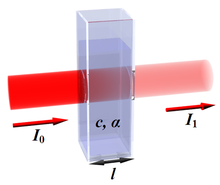
\includegraphics[width=\marginspace]{figures/beer.png}
\end{center}
\emph{\footnotesize{Light passing through a sample cavity is attenuated by the absorbers within the solution. Courtesy Wikipedia.}}
\label{fig:microtiter}
\end{wrapfigure}

This is known as the Beer Lambert law. The law relates the loss of light in a
material to the concentration of absorbers inside that material based on the
amount of light passing through the absorber and the properties of the absorber
itself.  While this version of the  law is formulated using a natural logarithm, it is also common to see the law in a base ten format \cite{Hollas:2004uh}.

The Beer-Lambert law can also be used for multiple absorbers in a single material by simply adding the absorption coefficients of all of the absorbers together.

\begin{align*}
  A(\lambda) = l\sum\alpha(\lambda)_i
\end{align*}

While the Beer-Lambert law is simplistic, it falls prey to some simple sources of interference, including the following \cite{Skoog:1994wg}.
\begin{itemize}
  \item Little tolerance to other light loss pathways such as scattering.
  \item Optical saturation limits, where the absorbers cannot accept any more light due to already being in an excited state.
  \item Requires a homogeneous mixture of the absorbers.
  \item A collimated light sources to allow the path length to be constant.
\end{itemize}

\marginpar{Pulse oximeters can be used together with other technologies to
acquire physiological parameters across the entire body: see the Esoma project.
\url{http://www.rdodesigns.com}}

Despite these limitations, the Beer-Lambert law has found many uses in modern
analytical devices. One of the most familiar devices is a pulse oximeter, which
measures blood oxygenation levels in a patients blood. This is done by passing
light across the patient's index finger to see how much light was lost to
oxygenated and deoxygenated blood. The concentrations of these two types of
blood can then be used to derive the total body blood oxygenation levels to a
high degree of accuracy \cite{Wukitsch:1987tb}.



\subsection{Electronic Transitions}\label{subsec:elec_trans}

\marginpar{In this section will be talking about atoms but the concepts apply to molecules as well}

Knowing how to measure concentration using absorption measurements is useful,
but with broadband light sources it is possible to measure absorption events
due to several different electronic transitions within an absorber. This
information can then be used for a better understanding of the absorber in
question, and allow properties such as fluorescence lifetimes to be measured
from absorption events \cite{Werts:2002fs}.

In addition to experimentally probing an absorber to determine its electronic
structure, it is possible to theoretically guess both the energy required for
an electronic transition and where it will take place. This is often done
through Hartree-Fock approximations to determine the energy required for an
electronic transition \cite{Szabo:1996tu}, and Judd-Ofelt theory to guess the
absorption strength at that transition \cite{Judd:1962uq}.



\section{Complications in Absorption Spectroscopy}\label{sec:comp_abs}

While absorption spectroscopy can be applied to a variety of materials, there
are several phenomenon that reduce the potential applicability of the
technique. Two of these phenomena -- spectral line broadening and scattering
losses -- are discussed below.



\subsection{Line Broadening}\label{subsec:line_broad}

Under theoretical conditions, with perfectly still particles, absorption lines
would be exceptionally thin due to the fact that only certain quantised energy
packets would create an excited condition. In reality, absorption lines are
quite broad, on the order of a few nanometers in liquid \cite{Hollas:2004uh}.
This broadening occurs due primarily to two factors: the Doppler effect
and collision based broadening (also known as Lorentzian or pressure based
broadening) \cite{Olivero:1977ul}.

Doppler based broadening is the Doppler effect applied to moving particles.
A particle at rest will see a incoming photon of light having a certain
frequency. If this particle is instead moving away from the photon, the
frequency of the light will appear to the particle as a lower frequency than
when the particle was standing still, as the distance between the crests and
troughs of the wave is greater in the particles inertial frame. Conversely,
if the particle is moving towards the photon, the photon will appear to have
a higher frequency than when the particle was standing still. The particle
in question will still absorb at the same quantised energy, but now photons
with greater and lesser energy than the transition will appear to have the
correct energy, broadening the range of wavelengths that the particle absorbs
\cite{Fox:2006uy}.

Collision based broadening leads to a similar effect of a broadening of
acceptable photon energies, but through a pressure pathway. As particles in
the solution collide into each other, they acquire some energy that puts them
in a state higher than their ground energetic state. As such, less energy is
required by the photon to cause an absorption event, leading to the absorption
of lower energy photons \cite{Ngo:2012jk}.

Both of these effects alter the absorption peaks in a spectra of an
aqueous absorber, leading to very broad absorption peaks. These broadening
effects lead to difficulty in the analysis of the acquired spectrum in two
different ways.

First, if two absorption peaks are too close together, they will appear as
one combined absorption peak. This causes a loss of information, as it is
impossible in most cases to calculate the absorption due to one transition
versus its nearby neighbor \cite{Fowles:1975wg}. This type of loss of
information does not often occur for electronic transitions in a molecule, as
the accepted electronic transitions are spaced out energetically due to the
higher energy required to jump to a higher molecular orbital. The collision of
absorption signals does become a problem when multiple absorbers are present
in a solution, often leading to signals that cannot be decoupled from one
another.

The second difficulty broadening causes in analysis is the understanding of
the hyperfine structure of certain transitions. When an electron is excited to
a higher energy state, it can often be excited into a multiplet of rotational
and vibrational energy states \cite{Levine:2008uh}. On top of this, many
degenerate energy states can exist for one transition, which will only be seen
if an external electric or magnetic field causes the fields to split (via
the Stark effect) \cite{Condon:1951wd}. These different states are separated
from each other by minute differences in energy, making the transitions
unobservable in liquid solutions.



\subsection{Scattering Losses}\label{subsec:scattering}

\begin{wrapfigure}{o}{\marginspace}
\begin{center}
  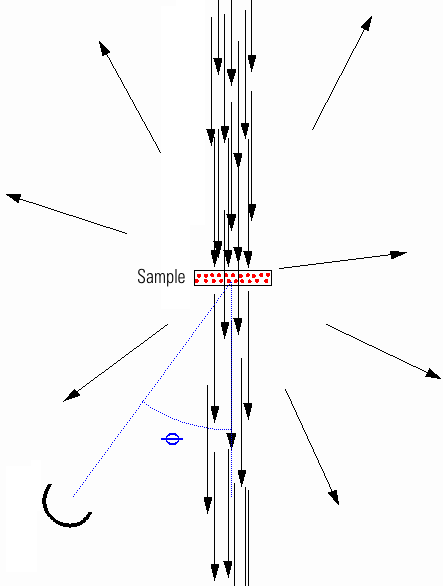
\includegraphics[width=\marginspace]{figures/scatter.png}
\end{center}
\emph{\footnotesize{Scattering of photons from molecules in a sample. Courtesy Wikipedia}}
\end{wrapfigure}

In addition to broadening schemes, liquid absorption measurements fall victim
to the fact that Beer-Lambert type experiments cannot differentiate between
light lost due to scattering versus due to absorption.  In gas phase
measurements, scattering is often not a concern due to the density of objects
on which scattering could occur. However, with the higher probability of a
photon being scattered in liquids, the assumption that scattering plays a minor
role in light loss is no longer valid. This leads to higher baseline error and
requires higher light intensities to be pumped into the absorbing medium, since
much of the  light will be lost just by trying to traversing the cavity.

The loss of light due to scattering also restricts the types of solutions that
can be observed. If a solution is turbid it may be difficult to find a powerful
enough light source that can push enough photons through the sample to detect
any light after the sample medium. Similarly, a solution that becomes turbid
during a measurement through either chemical reactions or colloidally will be
an impractical candidate for absorption measurements, as the loss of light due
to scattering changes over the time of the measurements. This turbidity problem
becomes especially pronounced in experiments designed to determine reaction
kinematics, as the absorption measurements over time will not be comparable due
to the shifting noise caused by scattering.

\marginpar{While a change in the normal index of refraction does not alter
absorption effects, a change in the complex index of refraction does cause
changes in absorption events due to the imaginary term}

Light can also be lost due to changes in the index of refraction for the
solution. Many gas solutions are dilute enough that the index of refraction of
the medium does not change significantly between measurements and blanks. This
scenario is different in liquids, where the index of refraction can change
significantly depending on the solvent and even the concentration of the
solute. This change in the index of refraction does not alter the absorption
events themselves, but presents a difficulty when attempting to align an
optical system. In the simple case of a single pass absorption, this effect can
lead to a loss of signal due to divergent beams that is dependent on the
wavelength, leading to a nonlinear error in the observed absorption spectrum.
In multipass systems, the misalignment of an optical cavity due to the change
in the index of refraction can preferentially support and discourage certain
modes, leading to a similar nonlinear error in an absorption spectrum. These
divergent beam problems can be mitigated by using a collimated source that
enters perpendicular to the cavity walls, negating the effects of the changes
in refraction. Unfortunately, in practice it is quite difficult to create a
perfect perpendicular alignment, and some error will always be present.

Even though broadening, scattering and changes in the index of refraction can
cause high and nonlinear errors to occur in absorption measurements, these
effects can be mitigated by a careful choice of the layout of the optical
system and the choice of the analyte. Experiments that measure clear solutions
with minimal changes in index of refraction are good candidates for absorption
spectroscopy, given that the experimenter does not require an understanding of
the hyperfine structure of the absorber in question.



\section{Broadband Absorption Spectroscopy}\label{sec:broad_abs}

The ideas gleaned from the Beer-Lambert law are dependent on wavelength of
light used to probe a material. As such, Beer-Lambert law is often used with a
single monochromatic light source and a simple photodiode as a detector.
However, there are many spectroscopic analyses that are not only concerned with
the absorption signal at a peak wavelength but in the shape of the transition
itself. Some applications require several absorption signatures to be measured
from a single sample. For these systems, absorption signals from a range of
wavelengths is required. Luckily, there are several methods that allow
experimenters to acquire absorption measurements at several wavelengths, both
sequentially and simultaneously.



\subsection{Tunable Diode Lasers}\label{subsec:tdl}

\begin{wrapfigure}{o}{\marginspace}
\begin{center}
\includegraphics[width=\marginspace]{figures/diode_laser.pdf}
\end{center}
\emph{\footnotesize{A simple laser diode, where the red ellipse represents the emission of light. Courtesy Wikipedia}}
\end{wrapfigure}

One common method for acquiring broadband signals is to use a light source
known as a \acf{TDL}. \ac{TDL} sources are diode lasers that are tunable
through either current or temperature \cite{May:1998ue}. Since temperature is
difficult to control, current is varied to sweep the frequency of the laser
light. This variation technique is used in \ac{TDLAS}, where the laser is
tuned to a particular frequency, an absorption measurement is taken, and then
this process repeats.

An advantage of \ac{TDLAS} over some of the other broadband techniques is that
the resolution of the instrument is dictated by the laser line width, which
provides sub nanometer resolution \cite{Berden:2009wk}. As a corollary, this
technique can use a simple photodiode or \ac{PMT} to acquire the intensity of
the laser light, instead of using a grating to disperse the light across a
detector.

\marginpar{A good discussion of wavelength modulation spectroscopy in the form
of an aircraft hygrometer can be found in \cite{May:1993tu}.}

Even though this method is simple to implement and cost effective, it suffers
from two major drawbacks. The first is that the broadband acquisition is done
sequentially, which creates an acquisition time versus resolution and spectral
range trade off to consider. \ac{TDLAS} also suffers from a problem inherent
to standard single pass absorption techniques, which is that the instrument
must detect a potentially small intensity change on top of a large background
signal. However, this second intensity problem can be mitigated through the use
either \ac{WMS} \cite{Reid:1981vq} or \ac{FMS}.



\subsection{LEDs}\label{subsec:led}

Another light source that has interesting potentials for broadband absorption
spectroscopy are \acp{LED}. \acp{LED} can provide light at a broad range of
frequencies and at high output intensities. \acp{LED} can even come in white,
infrared and ultraviolet variants, which can be used directly in absorption
spectroscopy. Best of all, these sources are extremely cheap to produce, making
\acp{LED} attractive sources for use in compact, inexpensive and portable
equipment.

Unfortunately \acp{LED} are quite difficult to use for absorption
spectroscopy.  \acp{LED} are incoherent sources, and as such it can be
difficult to couple the light from an \ac{LED} into a
cavity \cite{Seetohul:2009du,Islam:2007ea}. Even if light is successfully
coupled into the cavity containing absorber molecules, the amount of light
lost attempting to create a collimated beam often leads to minuscule fractions
of the light reach the detector.


\begin{wrapfigure}{o}{\marginspace}
\begin{center}
\includegraphics[width=\marginspace]{figures/led.pdf}
\end{center}
\emph{\footnotesize{A diagram of an \ac{LED}, courtesy Wikipedia.}}
\end{wrapfigure}

An additional complication from \acp{LED} is that once the broadband light
arrives at a photodetector the light must be separated into its constituent
wavelengths to acquire the broadband signal.  Two problems occur from this. If
one uses a spectrophotometer with a adjustable slit and moving diffraction
grating, then the signal acquired on a photodetector must be done
sequentially.  This increases the acquisition time, and suffers from reduced
spectral resolution when compared with a \ac{TDLAS} experiment due to the
limiting factor of the resolution being the diffraction grating. One can
mitigate the acquisition time conundrum by using a line detector instead of a
single photodetector, but this carries with it a second problem: the
acquisition, while happening simultaneously across several wavelengths, is
often more difficult to align and can lead to a lower spectral resolution as the line detectors elements have finite size and spacing.



\subsection{Supercontinuum Lasers}\label{subsec:super}

Supercontinuum laser light sources combine the advantage of a broadband source
with a tightly collimated beam and high output powers. This makes alignment
much simpler than in the case of an \ac{LED} with the added benefit of low
power loss while coupling into a absorbing medium.


\begin{wrapfigure}{o}{\marginspace}
\begin{center}
  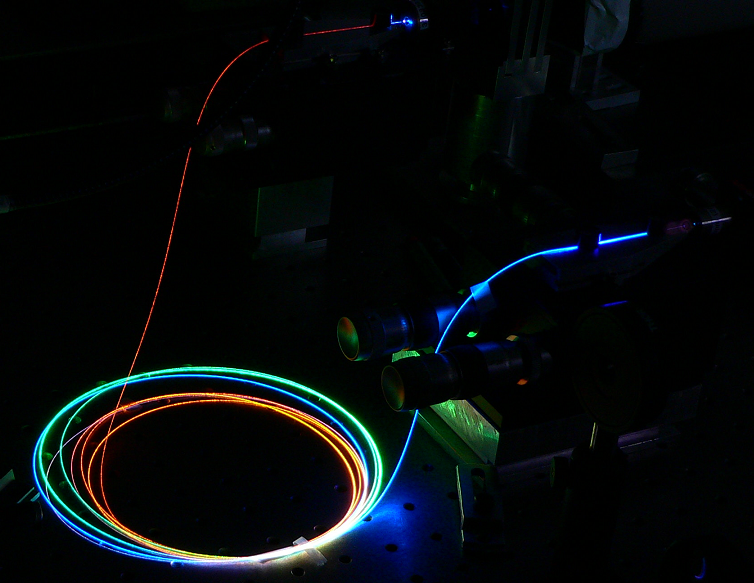
\includegraphics[width=\marginspace]{figures/supercontinuum.png}
\end{center}
\emph{\footnotesize{a Nd:YAG laser pulse being transformed into a supercontinuum by injecting the pulse into a photonic crystal fibre. Courtesy Wikipedia.}}
\end{wrapfigure}

While supercontinuum sources build on the advantages of \acp{LED}, they
introduce problems of their own. The most practical problem is the cost of
supercontinuum sources, which can cost upwards of \pounds40,000 at the time of
writing. Secondly, supercontinuum sources are prone to intensity fluctuations
over time and wavelength, and as such introduce higher error in an absorption
measurement.  Finally, these sources are not robust like \acp{LED} or
\acp{TDL}, and therefore cannot be taken outside of the laboratory.



\section{Multipass Techniques}\label{sec:multipass}

Besides acquiring broadband signals, it is also desirable to increase the
resolution of detectable concentrations and the lower limits of detection.
According to the Beer-Lambert law \eqref{eq:beer}, the simplest way to increase
the detection resolution is to increase the path length of the cavity. However,
as increasing the length of the sample cavity is often impractical due to
constraints of space or limitations of the absorbing molecules, it is common to
see optical designs that pass over the same sample several times. This is known
as a multiple pass technique. Two major versions of this technique are outlined
below.



\subsection{Multipass Cells}\label{subsec:herriott}


\begin{wrapfigure}{o}{\marginspace}
\begin{center}
  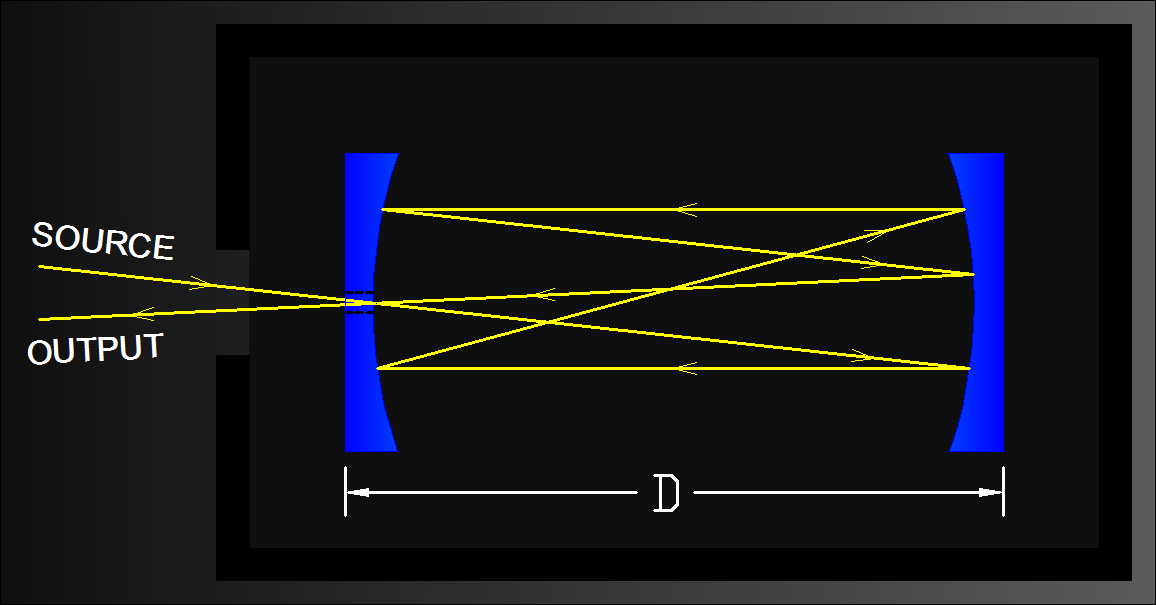
\includegraphics[width=\marginspace]{figures/herriott.png}
\end{center}
\emph{\footnotesize{A Herriott cell, shoring the path of light within the cell. Courtesy Wikipedia.}}
\end{wrapfigure}

One simple way to traverse a sample multiple times is to build a cavity with
two mirrors on either end that reflect the light back and forth through the
sample. It is possible to find mirrors that allow light to enter through a hole
in one mirror, bounce around a few times inside the cavity, and then exit
through a hole in the second mirror. These cavities are known as Herriott
cells, and they provide a simple and convenient way to increase the path
length \cite{Engel:2007va}. In the resulting measurement, the effective path
length is the distance across the sample multiplied by the number of passes,
making it possible to increase the resolution by a couple orders of magnitude.

These cells, while providing increased resolution, can be difficult to align.
In addition, Herriott cells can be misaligned once in place by accumulation of
particulates on the mirror surfaces.



\subsection{Optical Cavities}\label{subsec:cavity}


\begin{wrapfigure}{o}{\marginspace}
\begin{center}
  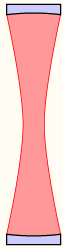
\includegraphics[height=100pt]{figures/cavity.png}
\end{center}
\emph{\footnotesize{An optical cavity and the light propagation inside using plano-convex mirrors. Courtesy Wikipedia.}}
\end{wrapfigure}

A similar approach to  Herriott cells is to use an optical cavity akin to a
laser cavity, except where both mirrors are only partially reflective. In such
a cavity, light leaks in through the first mirror, traverses across the sample
\emph{along the same path every pass} as the light bounces between the mirrors,
and then exits through the second mirror \cite{Berden:2009wk}. This method has an advantage over
Herriott cells in that the increase in the path length can be several orders of
magnitude higher if high reflectivity mirrors are used. For example, for
mirrors of reflectivity $R=0.999$, the increase in the path length will be
$(1-R)^{-1} = 1000$, which is a higher gain than most Herriott cells can
achieve.

Unfortunately these cavities are also difficult to align, as the input beam
must be perpendicular to the axis of the cavity. In addition, this method
requires a higher initial input intensity as a significant amount of light is
reflected when attempting to enter the cavity. Optical cavities introduce an
error due to the change in reflectivity of the mirrors based on wavelength that
must be measured and accounted for in the absorption spectrum. Finally, this
method can be more expensive than other multipass techniques, as high quality,
high reflectivity mirrors are expensive.

\marginpar{The mirror reflectivity curves depend on the alignment of the cavity
as well as the mirror surfaces. As such, it is not possible to use mirror
transmission curves provided by a manufacturer \cite{Berden:2009wk}.}



\section*{Chapter Review}

It is clear that absorption spectroscopy, based on the Beer-Lambert law
\eqref{eq:beer}, can be utilised to provide valuable information about a
material non-invasively. While the standard single pass technique can and has
been used successfully in commercial devices like pulse oximeters, there is
still a desire to increase the resolution of such systems to acquire
information on unlikely electronic transitions or minute traces of absorbers.
Augmentations that increase the path length and wavelength range of the
measured spectra are commonly in use today, and prove a cornerstone to
sensitive analytical techniques. In the coming chapters these improvements to
single pass absorption spectroscopy will be put to use to detect trace
concentrations of chemicals such as rhoadmine 6G and to analyse absorption
signatures of aqueous europium ions.

\chapter{Broadband Cavity Enhanced Absorption Spectroscopy}\label{ch:bbceas}

\acf{BBCEAS} is a recently devised experimental technique that uses the cavity
enhancement factors of \ac{CRDS} without requiring fast and sensitive detectors
to determine the ringdown time \cite{Berden:2009wk}. This chapter  will discuss
how to create a \ac{BBCEAS} instrument, the advantages and limitations of this
spectroscopic technique, and the design of the optical system used in this
report.



\section{Broadband Cavity Enhanced Absorption Techniques}\label{sec:bbceas}

\acl{BBCEAS} setups are very similar to their \ac{CRDS} brethren. In both
cases, light that enters the optical cavity passes through the sample a certain
number of times before exiting the cavity, after which the light is measured
using a wavelength dispersed detector. Unlike \ac{CRDS}, where the ring down
time is measured directly, \ac{CEAS} uses the fact that, with a continuous wave
source, the time integrated light intensity output from the cavity is directly
proportional to the ringdown time of the light within the cavity
\cite{Engeln:1998uq}.  Knowing this relation, it is possible to derive
following function for the absorption coefficient from the ring down equation \cite{Berden:2009wk}.

  \begin{align*}
    \alpha(\lambda) =
    \left(\frac{I_0(\lambda)}{I(\lambda)}-1\right)\left(\frac{1-R(\lambda)}{d}\right)
  \end{align*}

In this equation, $\alpha$ is the absorption coefficient (in \icm),
$\frac{I_0}{I}$ is the ratio of the intensity of the light passing through the
cavity with a blank and with the absorbers, $R$ is the reflectivity of the
mirrors used and $d$ is the length of the sample cuvette (in cm). It is
important to note that $d$ is not necessarily equal to the length of the
cavity, as it is more common to place the cuvette inside the open cavity
instead of soiling the mirrors with different solutions.

To take full advantage of this equation, \ac{BBCEAS} uses a broadband light
source to acquire information about the absorbers in a solution at many
wavelengths simultaneously. When the broadband source is incoherent, this
technique is known as \acf{IBBCEAS} \cite{Berden:2009wk}. A relatively new
technique uses a supercontinuum laser source instead, and is known as
\acf{SC-CEAS} \cite{Kiwanuka:2010bj}.



\subsection{Advantages}\label{subsec:bbceas_adv}

\acl{BBCEAS} has several advantages over its sibling techniques. Regular
\ac{CRDS} or \ac{BBCRDS} require fast, expensive light sources and detectors to
accurately acquire ring down signals. This cost and complexity does not exist
in \ac{BBCEAS}, as modest spectrometers and light sources can be used.
Additionally, this technique can be used to acquire high bandwidth spectrum,
which is practically limited by the mirror dielectric coatings
\cite{Islam:2007ea}.

Other broadband techniques exist that provide a higher spectral resolution, but
require a laser source such as a \acl{TDL}. These require special driver
circuitry and cannot capture the entire bandwidth in one acquisition event.

Finally, the simplicity of the technique is perhaps its most engaging feature.
\ac{BBCEAS} setups are not difficult to understand, and only require a modest
training in optical alignment to achieve significant improvements over standard
single pass techniques.



\subsection{Limitations}\label{subsec:bbceas_limits}

While there are many benefits to \ac{BBCEAS} for acquiring absorption spectrum
of a solution, the technique trades simplicity and broadband acquisitions for
higher error, lower limit of detection and potentially low spectral
resolution.

\marginpar{The causes of error in \ac{CEAS} systems is described in
Section~\ref{subsec:ceas_error}}

An obvious limitation is the absorptivity resolution of the technique, which is
limited by the noise of the detector. Many \ac{BBCEAS} setups use a \ac{CCD}
camera combined with a diffraction grating to detect the intensity of light
coming out of the optical cavity \cite{Berden:2009wk}.  \acp{CCD} do not have
the ability to detect tiny differences in light intensity due to the noise
inherent to the detector. This effect can be minimised by the use of a cooled
\ac{CCD}.

\acp{CCD} contain an addition pitfall in that are not as sensitive as the
photodiodes or \acp{PMT} used in \ac{CRDS}, which limits the ability to detect
minute changes in concentration. This detection sensitivity can be offset by
the use of an \ac{EMCCD}, but these detectors are expensive at the present
time, which defeats part of the original advantages of \ac{BBCEAS}. Even if one
was to use an \ac{EMCCD}, the sensitivity of the setup is unlikely to be that
accurate due to fluctuating light sources and, in some published papers,
unknown reflectivity curves \cite{Islam:2007ea}.

\marginpar{For a discussion on the advantages and disadvantages of \acp{TDL}
see Section~\ref{subsec:tdl}}

While \ac{TDL} based broadband techniques have longer acquisition times, they
easily outperform most \ac{BBCEAS} techniques in terms of spectral resolution.
This is due to the narrow linewidths of a \ac{TDL}, which is accurately
known and imaged onto a photodiode. \ac{BBCEAS} is limited in spectral
resolution by a diffraction grating and, more importantly, the focusing optics
and irises used in the spectrometer. It is not uncommon to see a high
resolution spectrum taken with a \ac{TDL} having a spectral resolution lower
than 0.1nm \cite{Wieman:2000vd}, whereas a grating spectrometer has a spectral
resolution on the order of nanometers \cite{Kiwanuka:2010bj}.

Another limitation is that this technique requires a calibration, or ``blank'',
sample to be measured before the spectrum of an analyte can be taken. This
causes higher error in the absorption measurements as the error in acquiring
the blank spectrum is added to the error of acquiring the sample spectrum. The
use of a blank is also an annoyance factor, where an extra step must be taken
to acquire the spectrum of the blank and then flush it out of the cavity with
the sample in question.

Finally, without the use of a device such as a \ac{CCD} streak camera, the
temporal resolution is limited by the exposure time of the \ac{CCD}. It is
terribly difficult to measure the change in a chemical reaction that occurred
on the order of milliseconds using a \ac{CCD}, whereas this type of measurement
would be trivial to watch with the nanosecond temporal resolution of the
\acp{PMT} used in \ac{CRDS}. Even a streak camera can obtain nearly this
temporal resolution, although not without significant cost and construction
time \cite{Velten:2011vq}.



\subsection{Considerations for BBCEAS in Liquid Medium}\label{subsec:bbceas_liq}

The advantages and limitations of a technique must be put into context
to determine its value for a particular experimental setup. In
chapter~\ref{ch:cal} and \ref{ch:europium} the \ac{BBCEAS}
setup laid out in this chapter is used to detect absorbers in liquid
solutions. As such, the low spectral resolution obtained with a modest grating
spectrometer is good enough for the wide features present in liquid solutions
(with rare exceptions, noted in section~\ref{sec:eu_measurements}).
Additionally, the samples measured in this report do not vary over time, and
hence the low temporal resolution is unimportant.



\section{Algorithms for BBCEAS}

The basic procedure for a CEAS experiment is to do the following.

\begin{enumerate}
  \item Setup the instrument and perform all of the alignment with a blank
        inside the sample cuvette.
  \item Perform a measurement of the intensity per wavelength leaving the
        cavity with the blank inside the cuvette. This can be done a number of
        times $n$ to acquire a mean intensity $I_0$ and its standard deviation
        $\sigma_{I_0}$
  \item Perform the same measurement with the absorber inside the cuvette,
        acquiring the mean intensity $I$ and its standard deviation
        $\sigma_{I}$.
\end{enumerate}

Once this information has been gathered, one uses a \ac{BBCEAS} equation to
calculate the absorption coefficient $\alpha(\lambda)$, usually in \icm.
However, there are several ways of performing this calculation, as described
below.



\subsection{BBCEAS Equation}\label{subsec:bbceas_eq}

\marginpar{For all equations in this section, be careful of when $I = 0$.}

While all \ac{BBCEAS} setups perform experiments in the same manner, where an
intensity spectrum of a blank and with the solute are taken, there are four
different equations in use in the literature to calculate absorption
coefficient values \cite{Mazurenka:2005fh}. The most common one is shown below

  \begin{align}
    \alpha(\lambda) = \left(\frac{I_0(\lambda)}{I(\lambda)}-1\right)\left(\frac{1-R(\lambda)}{d}\right)\label{eq:ceas_std}
  \end{align}

\marginpar{$\lambda$ dependence is implied for $\alpha$, $R$, $I_0$, and $I$ in
the following derivations}

This equation is a result of the cavity ring down equation at steady state,
under the assumptions that the mirror reflectivity $R$ tends to 1 and that the
absorption coefficient tends to nearly zero. Due to these assumptions, this
technique is best served for the analysis of gas phase solutions, although it
has been shown to be applicable over nearly all experimental conditions that
one would want to run \cite{Mazurenka:2005fh}.

A second equation in use in the literature does not make the assumptions that
$R \to 1$ and $\alpha \to 0$ due to the fact that it is derived from a
geometric sum instead of an indefinite integral \cite{Fiedler:2003db}. This
equation is slightly more complicated.

  \begin{align}
    \alpha = \frac{1}{d}\left|\ln\left(\frac{1}{2R^2}\left(\sqrt{4R^2+\left(\frac{I_0}{I}(R^2-1)\right)^2} + \frac{I_0}{I}(R^2-1)\right)\right)\right| \label{eq:ceas_geo}
  \end{align}

While this equation appears to be unwieldy, it is not more computationally
complex than the standard equation. However, the lack of assumptions for
the geometrically derived \ac{BBCEAS} equation makes it a better candidate
for analysis since one does not have to worry about the cases where the
mirror reflectivity is low (such as those that would be used in a low cost
instrument) or for high absorption coefficients.

In this report, the following equation is used. \marginpar{Equation \eqref{eq:ceas_geo_mod}, \eqref{eq:ceas_err_std} and \eqref{eq:ceas_err_geo} have be derived by the author.}

\begin{align}
    \alpha = \frac{1}{d}\ln\left(\frac{1}{2R^2}\left(\sqrt{4R^2+\left(\frac{I_0}{I}(1-R^2)\right)^2} - \frac{I_0}{I}(1-R^2)\right)\right) \label{eq:ceas_geo_mod}
\end{align}

This equation is a modification of the geometrically derived equation. First,
the absolute value operator was removed. Since negative absorption coefficent
values only occur when the intensity of the blank spectrum is higher than the
sample spectrum, it is easier to be able to note these abnormalities through
negative numbers. In addition, equation \eqref{eq:ceas_geo_mod} rearranges the
$R^2-1$ terms to $-(1-R^2)$ make the deviation of the error function simpler.
This modification can be done because $R$ is bounded to the real set
$(0,1)$. Both of these modifications can be done without loss of generality.



\subsection{Error calculation}\label{subsec:ceas_error}

\marginpar{See appendix for full error calculation derivation. In addition, the full software implementation and an discussion of potential caveats can be found in the appendix.}

With a \ac{BBCEAS} equation in hand, it is important to derive a way to
estimate the error in this equation. The standard way to calculate the minimum
level of detection (as well as the error) in a \ac{BBCEAS} is to use the
following equation, which applies for calculating the error from equation
\eqref{eq:ceas_std} \cite{Mazurenka:2005fh}.

\begin{align}
  \alpha_{\text{min}} = \left(\frac{\Delta
  I}{I_0}\right)\left(\frac{1-R}{d}\right)\label{eq:ceas_min}
\end{align}

In this equation, $\Delta I$ is the minimum detectable change in $I$.
Similarly, the limit of detection (LOD) is normally defined as three times the
standard deviation in $\alpha$ \cite{Islam:2007ea}.

\begin{align}
  \text{LOD}_{\alpha} = 3\sigma_{\alpha}\label{eq:lod}
\end{align}

These equations present two different problems.  One is the way in which the
minimum detectable change is defined. If the minimum detectable change is
defined as how confidently the experimenter can assume a new intensity value is
unique to an absorber, one would likely use something similar to the limit of
detection. Alternatively, one could define the minimum detectable change in
intensity as a function of the noise in the detector only, instead of through
the entire experiment (as one assumes all other sources to be constant).

\marginpar{For a discussion of how light source fluctuation introduces errors
in the observed spectrum, see \ref{subsec:laser_fluc}}

While the photodetector is often the main source of noise, the blanket
assumption of error due to the detector excludes the intensity fluctuations in
the light source in calculating $\alpha$. As such, this error is too generous
to the actual achievable sources of error in a \ac{BBCEAS} experiment.

The second problem with the error calculations is that the error in the blank
measurement is not taken into account. Equation \eqref{eq:ceas_min} assumes
that one has a constant for the intensity of the blank $I_0$. However, we know
that this blank has its own error due to the fact that the measurement
procedure is identical to acquiring the sample spectrum. As such, the common
error equation in the literature is generous in the minimum detectable
absorption changes, and does not reflect the actual sensitivity of the
instruments devised.

To alleviate the problems of the error associated with the intensity of the
source and that of the initial blank intensity measurement, one may consider a
more accurate method of attempting to calculate the absorption coefficient many
times \cite{Islam:2007ea}. However, this can be immensely time consuming to
acquire a statistically accurate dataset for many concentrations, and requires
many flushes of the liquid inside the cuvette (increasing the sample volume
costs).

\ac{BBCEAS} experiments can calculate a more accurate error by altering the
method of spectrum collection. When an experimenter collects data on the
intensity distribution of the blank and solution samples, they often take many
snapshots of this information and then average that data. However, if one
calculates the standard deviation of the intensity signals, then it is possible
to \emph{approximate} the standard deviation in $\alpha$ using the delta method
\cite{Casella:2002tp}. This leads to the following equations of error for
equation \eqref{eq:ceas_std} and \eqref{eq:ceas_geo_mod}, respectively.

    \begin{align}
      \sigma_\alpha = \left(\frac{\sigma_{I_0}}{I} +
             \frac{I_0\sigma_I}{I^2}\right)
            \left(\frac{1-R}{d}\right)\label{eq:ceas_err_std}
    \end{align}


    \begin{align}
      \sigma_\alpha = \left(\frac{\sigma_{I_0}}{I} +
             \frac{I_0\sigma_I}{I^2}\right)
            \left(\dfrac{1-R^2}{d}\right)\left(4R^2+\left(
                                     \frac{I_0}{I}(1-R^2)\right)^2
                                     \right)^{-1/2}\label{eq:ceas_err_geo}
    \end{align}

It is possible to calculate the standard deviation in $\alpha$ exactly, as a
measure of sanity, by comparing each of the intensity spectrum of the
blank against each of the intensity spectrum of the sample. However, this
quickly becomes computationally demanding. If one was to take 50
intensity spectrum of the blank and the sample, over 1024 pixel bins inside a
CCD camera, then one would calculate $\alpha$ more than 2.5 million times,
which would take a while even on modern computers.



\section{Optical Layout and Design}\label{sec:optical_layout}

\begin{wide}
\begin{figure}
\begin{center}
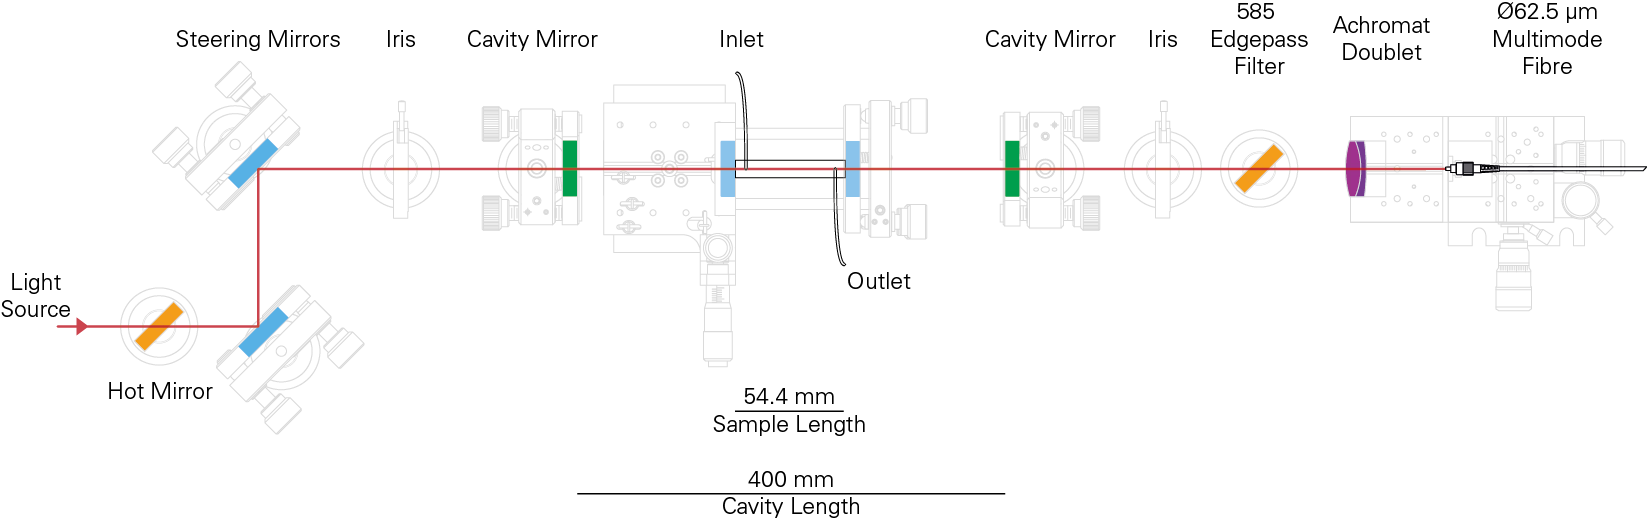
\includegraphics[width=500pt]{figures/bbceas_setup/bbceas_setup.pdf}
\end{center}
\caption{Optical setup for \ac{BBCEAS} experiments performed in this report}
\label{fig:optical_layout}
\end{figure}
\end{wide}


The optical layout for the system used in this report is nearly identical to
all \ac{BBCEAS} layouts \cite{Berden:2009wk}. The light source is a Fianium
\textsc{sc-450} supercontinuum pulsed laser source, with a high enough
repetition rate that it is treated like a continuous wave laser source in our
equations. After the source, an optical cavity is formed with mirrors of
reflectivity $R=0.99$. Finally, light exiting the cavity is coupled into a
multimode fibre and imaged using a custom built grating spectrometer.

Inside the cavity sits a cuvette compressed between two optical windows. This
cuvette holder is then mounted in a rotatable jig to make it easier to properly
align the cuvette with the cavity. This cuvette has inlet and outlet tubes,
which allow for the liquid inside to be changed. This setup was chosen over
mounting the cuvette directly to the mirrors \cite{Seetohul:2009ij} to prevent
the mirrors from accumulating particulates that would add significant noise to
the acquired spectrum.



\section{Potential Enhancements}\label{sec:bbceas_enhance}

While this setup works well, there are certain aspects of the instrument that
can be improved to make either a gain in sensitivity and/or in cost over the
current implementation.

\subsection{LED source}\label{sec:bbceas_led}

\marginpar{See Section~\ref{subsec:led} for a discussion of an \ac{LED} as a light source}

The supercontinuum light source is excellent for its low divergence and high
power properties over the visible range. However, such light sources are far
from cheap, and supercontinuum sources often have high fluctuations in
intensity over time that can be difficult to correct for without a reference
signal.

\acp{LED} offer an enticing visible light source alternative to supercontinuum
sources on the basis of their exceptionally low cost and stable output
intensity stability.

The current costs of high power \ac{LED} devices are on the order of only a few
pounds, and can be easily wired in series with a resistor in order to provide
stable light output. There is a potential complication in the power supplies
for high powered \acp{LED} because of power draw can be quite large.  However,
one can build highly stable current inputs into the \ac{LED} to aid in
stabilising the intensity output \cite{patent_const_current}. Additionally a
thermistor can be added to the \ac{LED} to create a closed loop system, where
the feedback from the thermistor assists in stabilising the light source over
time \cite{Wieman:2000vd}.

Once a stable output intensity is reached, the light from an \ac{LED} can be
fibre coupled into a multimode fibre. The light coming out of the fibre can
then be collimated to create a low divergence beam to be put into the cavity
\cite{Berden:2009wk}.  Other groups have shown that fibre-coupled \ac{LED}
light sources can be used for liquid \ac{BBCEAS} experiments
\cite{Islam:2007ea,Seetohul:2009du}, and that the setup for an \ac{LED} source
is relatively trivial.

An additional benefit of an \ac{LED} based light source is that the intensity
could be easily modulated by an external signal quickly. This could be used to
create lock-in type detection schemes, or to initiate a photochemical reaction
and watch the result through absorption spectroscopy.



\subsection{Non-fibre Spectrometer}\label{subsec:bbceas_no_fibre}

Coupling light into a multimode fibre can provide a convenient way to reroute
light to certain optical setups. The problem with coupling light into a fibre,
even a multimode fibre with a large diameter core, is that the loss of light at
the interface of the fibre is relatively high. Practically, lasers based setups
are unaffected by this coupling problem in \ac{BBCEAS} measurements as it is
often possible to reach higher output power levels with the laser to offset the
coupling losses.  There are even cases where one can saturate the absorber in a
\ac{BBCEAS} measurement if the light intensity is too high
\cite{Giuliano:1967hw}.

Incoherent light sources such as \acp{LED}, on the other hand, suffer from
problems of having wide, divergent emission profiles, which practically means
that these sources have limits on their intensity that cannot offset the fibre
losses. On top of this limit, losses for the incoherent source are higher than
the laser due to the larger spot sizes and diffuse nature of the light when
coupling into a fibre.

The current optical setup is convenient because different detectors can be
easily swapped to provide more accurate or faster acquisitions. But tests with
collimated \ac{LED} light sources in the \ac{BBCEAS} setup used in the report
have required integration times on the order of ten seconds, hampering the
effective use of \ac{LED} sources.

If the light coming out of the cavity is instead directed onto a transmission
grating, the losses due to the coupling would be removed, and much more light
would hit the detector. The loss of convenience would be greatly offset by the
ability acquire data at a faster rate and lower noise than in the case of the
fibre coupled spectrometer.



\subsection{Webcam}\label{subsec:bbceas_webcam}

While the current system uses a \ac{CCD} that costs much less than the
detectors in other \ac{CEAS} and \ac{CRDS} systems, the \ac{CCD} is still on
the order of a thousand pounds to buy at the time of writing. To further reduce
the costs of the \ac{BBCEAS} system, the detector can be replaced with the
\ac{CCD} from a web camera, which costs tens of pounds.

Replacing the \ac{CCD} with a web camera would bring the total costs, if one
uses low reflectivity dielectric mirrors, to potentially less than a hundred
pounds. The \ac{CCD} in a web camera is also incredibly tiny, and would allow
the entire \ac{BBCEAS} setup to be easily miniaturised into a portable device
using an \ac{LED} light source.


\section*{Chapter Review}

\ac{BBCEAS} is a promising new spectroscopic technique that can be utilised to
acquire signals from fiendishly small absorption cross sections. While this
method does contain some error, it can be readily quantified and accounted for
when analysing absorption spectra. While the current implementation of a
\ac{BBCEAS} provides usable results, some enhancements can be made to further
decrease the noise in the acquired signal and increase the intensity of the
light hitting the detector.

\chapter{Electronic Transitions of Europium}\label{ch:eu_theory}

Europium is a peculiar metal. Lanthanide metals have a complex
electronic structure consisting of an incomplete \textsl{4f} electron
shell, and many lanthanides, including europium, are highly reactive
\cite{Cooley:1946tv,Rard:1985tb}. These properties create a tricky
spectroscopic problem: europium has very low absorption cross sections in the
visible due to its electronic structure, and europium's reactivity means that
it is difficult to acquire lone europium to detect. This means that to analyse
europium in a solution it must be present at relatively high concentration in
a medium that europium does not react with.

\marginpar{Lower concentrations of europium can be measured in the UV.}

Using \ac{BBCEAS} it is possible to detect europium in a liquid sample at lower
concentrations than what is published in the literature.  The broad spectral
and simultaneous acquisition nature of \ac{BBCEAS} allows several spectral
features in the visible to be measured simultaneously.

While europium is challenging to characterise, it has a valuable
property: europium's photoluminescent quantum yield is nearly one
\cite{Scotognella:2009jo,Moudam:2009in, Bunzli:2005ic}, and the fluorescence
emission can be spectrally very narrow \cite{Werts:2002fs}. The quantum yield
is an important parameter in engineering uses for europium, yet this property
has not been explored well in the past due to the difficulty of extracting
information from fluorescence measurements \cite{Werts:2002fs}. By measuring
the absorption characteristics of europium using \ac{BBCEAS}, it is possible to
obtain a greater understanding of the fluorescence pathways and how to alter
them.

Europium also readily forms coordination complexes as both monodentate and
polydentate ligands
\cite{Kirby:1983cl,Sveshnikova:2000cr,Werts:2002fs,Bunzli:2005ic,Scotognella:2009jo,Moudam:2009in}. The fluorescence of europium, combined with a coordination complex, can be used
to create sensitive labels
\cite{Harma:2010dm,Pihlasalo:2010el,InstituteofBiomedicine:2011vt,Pihlasalo:2011ju,Pihlasalo:2012cq,Pihlasalo:2012en},
to create OLEDs with high spectral purity\cite{Moudam:2009in}, and as
luminescent solar concentrators\cite{Moudam:2009in,Wilson:2010hs}.

This chapter will explore the current understanding of europium's electronic
transitions and how to derive additional information such as quantum yields
and radiative lifetimes about europium complexes using \ac{BBCEAS}. At the
end of this chapter is a discussion about how it is possible to combine
\ac{BBCEAS} with europium complexes to create a highly sensitive protein
detection technique that can not only detect trace concentrations of proteins
but also indicate which proteins are in a solution.



\section{Theory of Lanthanide electronic transitions}\label{sec:theory_eu}

Lanthanide ions contain an open \textsl{4f} electronic orbital which leads to
many strange phenomena that are difficult to describe with standard quantum
mechanical models\cite{Wybourne:1968ez}. In the 1960s, researchers Judd and
Ofelt introduced simple assumptions to make the calculation of the electronic
wave functions simpler \cite{Judd:1962uq,Ofelt:1962kd}. Their simplifications
were successful in theoretically predicting the energy levels of different
electron configurations.

However, there exist electronic transitions that are still difficult to
understand because they are classically \emph{forbidden}. Some transitions are
forbidden due to a transition between two ground total angular momentum states
(noted as $ J=0 \leftrightarrow J'=0 $), while many others are forbidden due to
a change in the total spin $\Delta S \neq 0$. As such, these transitions must
occur due to higher order effects, such as electron configuration interaction
for the $^7F_0 \leftrightarrow ^5D_0$ transition \cite{Jankowski:1981es}, These
transitions have much weaker absorption cross sections than classically allowed
transitions.



\subsection{Predicting Energy Levels in Europium}\label{subsec:predict_eu}

\begin{figure}[t]
\begin{center}
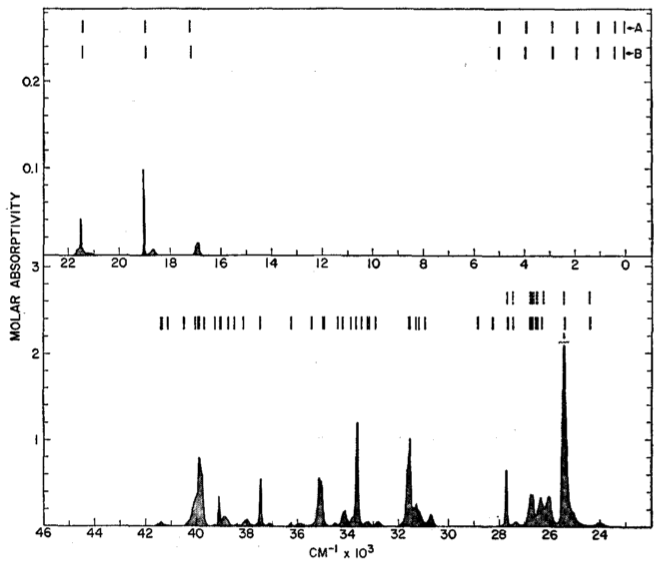
\includegraphics[width=\textwidth]{figures/eu_spec.png}
\end{center}
\caption[Aqueous Europium Spectrum from Literature]{The expected absorption spectrum of aqueous europium, taken directly from Carnall 1968\cite{Carnall:1968ch}. The weaker, forbidden transitions are mostly seen in the visible, there they have an order of magnitude lower molar extinction. The B line above the spectrum represents the theoretical electronic transitions calculated using \emph{ab initio} methods.}
\label{fig:eu_spec_theory}
\end{figure}

It is possible, using extensions to Judd-Ofelt calculations, to derive the
energy levels of the \textsl{4f} energy shell and the transitions from the
ground state of europium in different mediums
\cite{Carnall:1968ch,Carnall:1989fc,Richardson:1989vf,vanPieterson:2002hd}.

\begin{align}
  H = H_{\text{free ion}} + H_{CF} \label{eq:lan_ham}
\end{align}

%\begin{align*}
%H =\ & H_0 + \sum_{k=2,4,6} F^kf_k \\
 %& + \zeta(4f)A_{so} + \alpha L(L+1) + \beta G(G_2) + \gamma G(R_7)\\
 %& + \sum_{i=2,3,4,6,7,8}t_iT^i + \sum_{h=0,2,4}m_hM^h + \sum_{f=2,4,6}p_fP^f
%\end{align*}

This equation represents the free ion Hamiltonian of a lanthanide ion.
$H_{\text{free ion}}$ is the non-interacting electrons contribution (known as
the barycenter) \cite{Peijzel:2005jh}. Accurate quantum mechanical models of
the free ion term are available in the literature and can be easily solved
numerically on a computer \cite{Carnall:1989fc,Morrison:1988tw}.

One can then add perturbation terms to alter the Hamiltonian for use in
different solutions. For example, if the lanthanide is in a solid crystal
lattice, it is common to add

\begin{align*}
  H_{CF} = \sum_{k,q} B_q^k C_q^{(k)}
\end{align*}

which represents the radial $B$ and many-electron spherical tensor $C$ crystal
field interaction with the electron wave functions \cite{Peijzel:2005jh}.  Some
forbidden excited states of europium can also be understood through the
Wybourne-Downer mechanism, which accounts for spin-orbit interaction among
excited states and explicitly allows for $\Delta S = 1$ transitions to occur
\cite{Wybourne:1968ez,Downer:1988kz}.  Finally, Judd-Ofelt theory can be used
to estimate the transition intensities and branching ratios of absorption and
emission spectra, and therefore the natural radiative lifetimes
\cite{Werts:2002fs}.



\subsection{Measuring Radiative lifetimes of Europium Complexes using Fluorescence Emission}\label{subsec:rad_life}

The radiative lifetime of an electronic transition of an absorber can be
determined by its emission profile \cite{Werts:2002fs}. This is done through
the following formula.

\begin{align}
  \frac{1}{\tau_R} = \sum_JA_{J'J}\label{eq:nat_life_emiss}
\end{align}

In this formula, $A$ is the spontaneous emission probability of a particular
$J' \leftrightarrow J$ transition\marginpar{$A$ is also known as the Einstein
$A$ coefficient} (which is related to the area under the curve for that
emission peak), and $\tau_R$ is the ``natural'' radiative lifetime, which
is the lifetime of an electron in an excited state without interference
from systematic effects such as thermal quenching. Additionally, the
\emph{branching ratio} $\beta$ can be defined as the probability for an
excited electron to decay via a certain pathway $J_p$.

\begin{align}
  \beta_{J'J_P} = \dfrac{A_{J'J_p}}{\tau_R} = A_{J'J_p}\sum_J A_{J'J} \label{eq:branch_ratio}
\end{align}

For some absorbers, it can be difficult to measure all transitions
simultaneously, as some may be forbidden and hence extremely weak in comparison
to the allowed transitions. However, europium has a unique property that allows
its radiative lifetime to be determined from a single peak: europium contains a
single allowed magnetic dipole moment transition $^5D_0 \leftrightarrow ^7F_1$.
Magnetic dipole transitions are not affected by the solvent or complex that an
absorber is in, and hence this transition is constant \cite{Werts:2002fs}.
Using this peak, it is possible to measure the radiative lifetime using the
following equation

\begin{align}
  \dfrac{1}{\tau_R} = A_{MD,0}n^3\left(\frac{I}{I_{MD}}\right) \label{eq:nat_life_eu}
\end{align}

where $n$ is the refractive index of the solution, and the fraction
$\frac{I}{I_{MD}}$ is the ratio of the total area under the emission curve to
the area under just the $^5D_0 \leftrightarrow ^7F_1$ transition.

It is also possible, in cases where the absorption spectrum of a particular
luminescence transition is known, to calculate the radiative lifetime of the
transition \cite{Lewis:1945tp},

\begin{align}
  \frac{1}{\tau_R} = 2303 \dfrac{8\pi c n ^2 \nu^2}{N_A}\dfrac{g_l}{g_u}\int\epsilon(\nu)\,d\nu \label{eq:nat_life_abs}
\end{align}

where $\nu$ is the frequency of the transition, $\tfrac{g_l}{g_u}$ is the
fraction of electrons in the excited and ground state, and $\epsilon$ is the
molar extinction coefficient (in \iM\icm) of the transition.

\section*{Chapter Review}

Europium is a metal with a complicated electronic configuration that is not
fully understood at the time of writing. Theoretical investigations can
provide some indications to how europium ions will react to photons, but this
understanding is incomplete because of the strong response from ``forbidden''
transitions. Experimental tests must also be performed to attempt to create
an accurate model for europium's electronic transitions. Once the branching
ratios can be well predicted, their deviations from expected results can
be used to determine other particulates in a solution. This possibility is
discussed in chapter~\ref{ch:eu_exp}.

\part{Experiment}
\chapter{Calibrations}\label{ch:cal}

\acl{BBCEAS} has a simpler setup and lower cost in comparison to \ac{CRDS}, but
\ac{BBCEAS} does require a few calibration procedures in order to acquire
accurate absorption spectra. The basic calibrations that should be done with a
\ac{BBCEAS} instrument are: a measurement of the absorption limits where the
signal is linear, an analysis of the error of the detected intensity signal,
and the reflectivity of the mirrors used for the optical cavity.

To find the absorption coefficient values under which an \ac{BBCEAS} experiment
results in a linear correlation with concentration, it is common to test the
instrument using a strong absorber. One such absorber is rhodamine 6G, a dye
that can be used to create a laser \cite{Pappalardo:1970hi} or as a fluorescent
marker \cite{Gear:1974tf}.

The error in the detection of the intensity comes down to two important
sources: the error in the \ac{CCD} and the intensity fluctuation over time of
the light source. The intensity fluctuations are especially important, as it is
possible -- and in some cases, extremely likely -- for the intensity of the
light entering the cavity to change between the measurement of the blank and
the measurement of the sample. This fluctuation at best provides a false
understanding of the detection limit of the setup and, in the case of high
variability in the input source, silently modulates the absorption peaks in
acquired spectra.

Finally, the mirror reflectivity is required for any of the equations of the
absorption coefficient or its standard deviation. Giving a guess on the mirror
reflectivity at a particular wavelength based on the average mirror
reflectivity can lead to inaccurate absorption coefficient calculations and
alter the shape of the calculated spectrum \cite{Berden:2009wk}. This case is
more common than one may expect, as the multiple layers of thin films deposited
on the mirror's surface introduces characteristic ripples in the mirror
reflectivity as a function of wavelength \cite{Islam:2007ea}.

This chapter will discuss these calibrations for the stated problems to
characterise the \ac{BBCEAS} instrument used in this report.



\section{Limits of linearity using Rhodamine 6G}\label{sec:rhodamine}

There are two important considerations for regions where the concentration of
rhodamine correlates linearly with the concentration of an absorber. One
consideration is the calculation of absorption using $A = \alpha  l$, where $l$
is the path length when considering multiple passes through the cavity.  It is
possible to measure an $\alpha$ value that leads to an absorption of greater
than one, which has no physical meaning.

\begin{figure}
\begin{center}
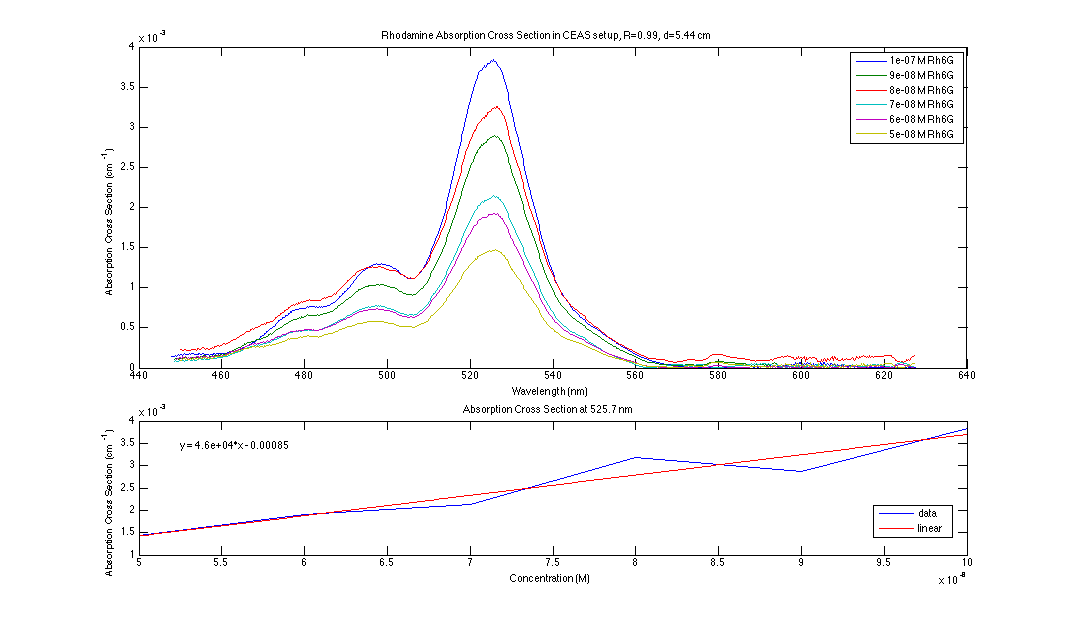
\includegraphics[width=\textwidth]{figures/Rh6G_absorption_cross_section_and_linearity}
\end{center}
\caption{Rhodamine 6G Spectrum from \ac{BBCEAS} measurement}
\label{fig:rh6g}
\end{figure}


While the upper bound to the linearity of the \ac{BBCEAS} equation is useful
for determining when experimental results may be strange, a tighter bounding
set is useful to determine what sorts of concentrations would be best measured
by the \ac{BBCEAS} technique. Unfortunately, the only way to measure where
absorption coefficients correlate linearly with concentration is to acquire
spectra from many different concentrations and plot the absorption at the peak
wavelength as a function of concentration. This is shown in
Figure~\ref{fig:rh6g_lin}.

\begin{figure}
\begin{center}
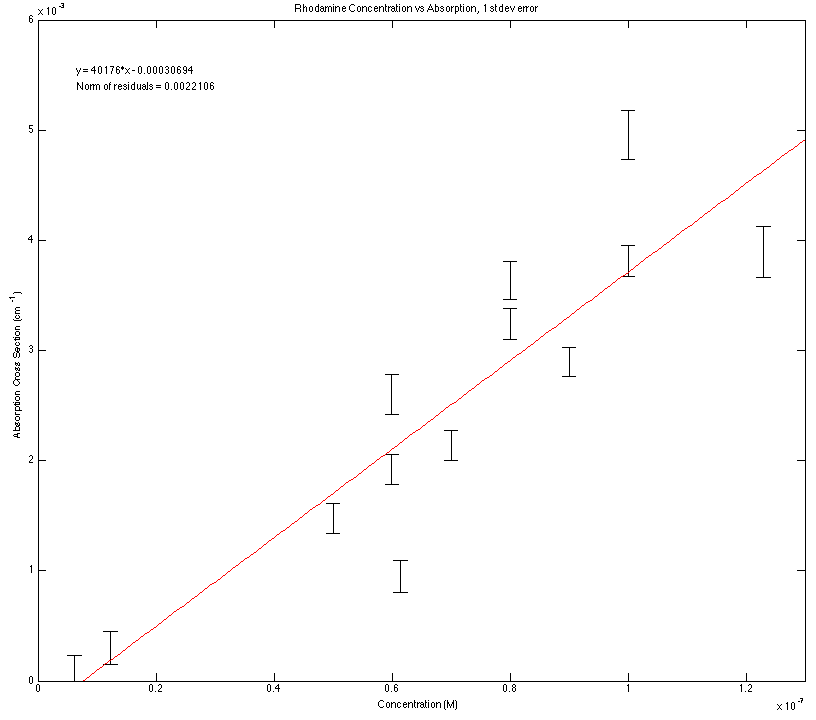
\includegraphics[width=\textwidth]{figures/rhodamine_concentration_vs_conc_linear.png}
\end{center}
\caption{Linearity in Rh6G \ac{BBCEAS} measurement. After this region, the collected data took on a cubic trend.}
\label{fig:rh6g_lin}
\end{figure}

\begin{figure}
\begin{center}
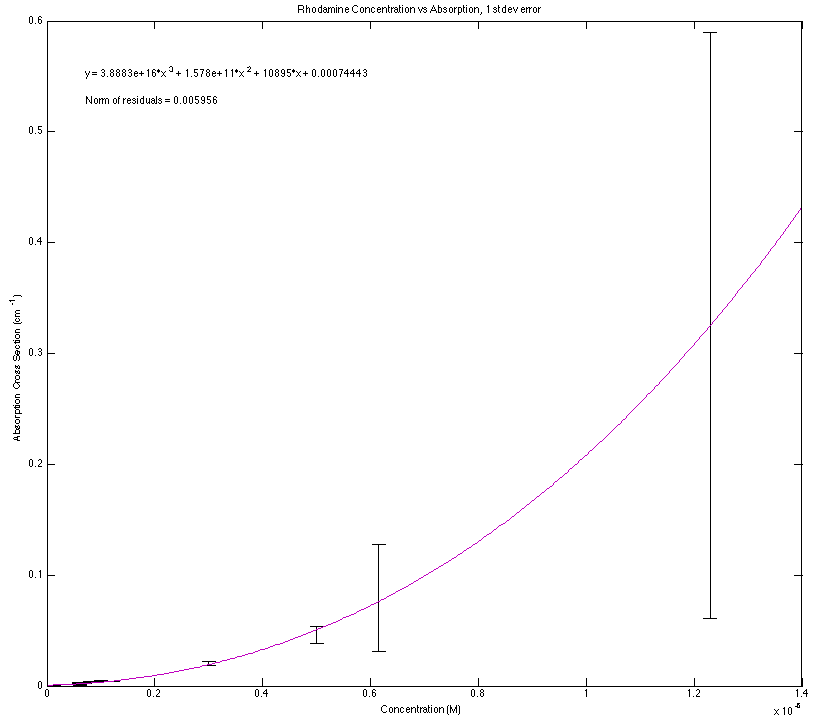
\includegraphics[width=\textwidth]{figures/rhodamine_concentration_vs_conc_non_linear.png}
\end{center}
\caption{Non linearity in Rh6G \ac{BBCEAS} measurement. The fitted line is a cubic trend.}
\label{fig:rh6g_nonlin}
\end{figure}

As can be seen in figure~\ref{fig:rh6g_nonlin}, the lower the concentration, the
better we can fit a linear regression to the data acquired. As such, a lower
bound is better defined as the limit of detection, instead of attempting to
extrapolate a linear function to below the noise levels of the instrument.

One problem with absorption spectroscopy techniques is that the dynamic range
is mainly dependent on the absorber. Strong absorbers will have smaller
concentrations where the calculated absorption coefficient is linear. Weak
absorbers have an advantage is greater detection ranges under this regime, but
suffer from a lower sensitivity to the concentration as small changes in
intensity correlate to larger changes in concentration, in comparison to strong
absorbers.

As a guide to the detectable concentration ranges, it is possible to calculate
the molar emissivity $\epsilon$ range of a \ac{BBCEAS} setup by dividing the
absorption coefficient value by the concentration it represents. Then, if one
knows the molar emissivity of an absorber it is possible to determine a rough
upper bound of the concentration limit of detection. Unfortunately many
substances of interest have unknown or poorly characterised absorption spectra
in terms of molar emissivity in the liquid phase, and there is no convenient
methods of determining valid concentration ranges.

\section{Intensity Fluctuations in BBCEAS measurements}\label{sec:light_fluc}

%% TODO Add section intro here.

\subsection{Intensity fluctuations due to light source stability}\label{subsec:laser_fluc}

\begin{figure}[h!]
\begin{center}
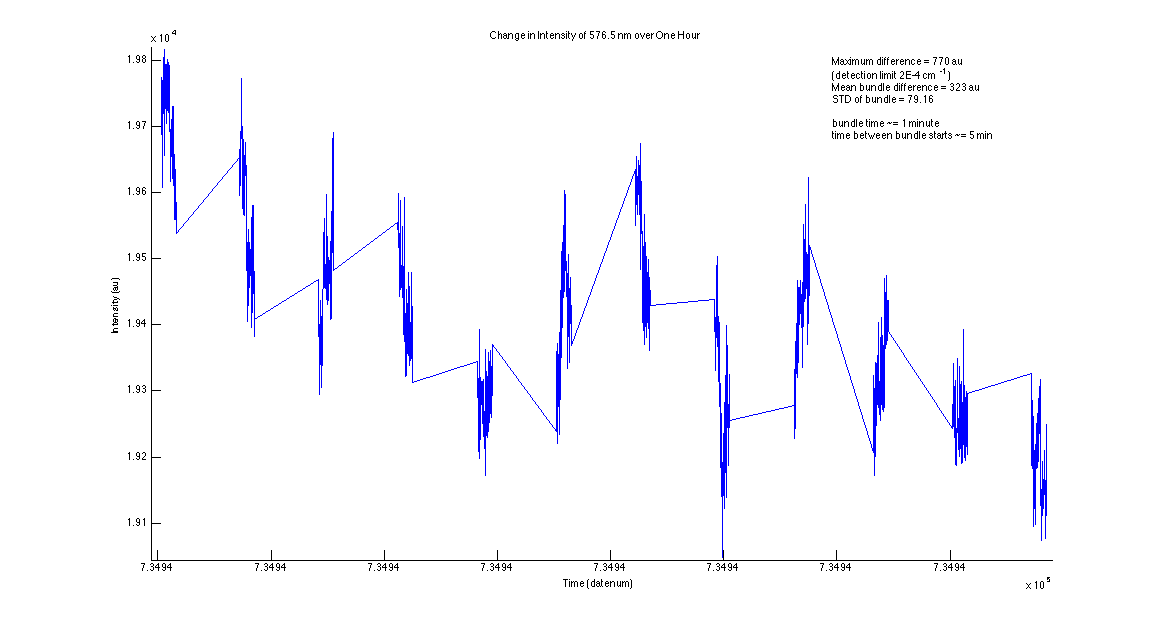
\includegraphics[width=\textwidth]{figures/change_in_intensity_of_576_5nm_over_one_hour.png}
\end{center}
\caption{Laser Fluctuation over time}
\label{fig:laser_fluc}
\end{figure}

\ac{BBCEAS} measurements, while based on \ac{CRDS}, do not share the benefit of
being immune to intensity fluctuations in the source \cite{Berden:2009wk}. This
is because \ac{CRDS} takes the measurement of the intensity of an individual
pulse of light, whereas \ac{BBCEAS} measures the average steady state ring down
intensity, which represents an average of the light intensity ring down times
across multiple pulses (for pulsed wave sources) or effectively infinite pulses
(for continuous wave sources).

Figure~\ref{fig:laser_fluc} illustrates the problem of light source
fluctuation. In this figure, each ``bundle'' represents approximately the
noise from the \ac{CCD}. If one considers this to bundle to represent the
width of the noise distribution due to the \ac{CCD}, then two different
phenomena can be seen from this figure.

The most obvious is that over time, the intensity error fluctuates in both a
high frequency range (mostly the \ac{CCD} noise) and a lower frequency. This
lower frequency is a result of the drift in the intensity of the output of the
supercontinuum laser. As such, it is simple to see that even a measurement
within five minutes of the blank sample is prone to intensity fluctuation
error.

The second problem with the laser fluctuation is that while most of the high
frequency noise is due to the \ac{CCD}, the stretching of the bundles suggests
that there is a high frequency noise component of the supercontinuum source as
well. This means that the fluctuation of the light source skews the
distribution due to the \ac{CCD} noise, sometimes broadening the width (such as
in the second, third and eighth bundles) and sometimes compressing the noise
distribution (as seen in the second to last bundle).

Combined, these two effects of the intensity fluctuation of the laser lead to
errors in calculating $\alpha$ due to drift between measurements and
$\sigma_{\alpha}$ due to fluctuations in $\sigma_{I}$ and $\sigma_{I_0}$. An
additional frustration arises when one considers that these fluctuations in
intensity are often wavelength dependent, so it is not simple to extrapolate
the error calculations in intensity from one wavelength to another.

If the blank and sample spectra are taken within a few minutes of each other,
these error effects are minimised, but still lead to unaccountable error in the
final absorption spectrum. Given that the calculation of the standard
deviations will take part of the high frequency noise into account, and the
fast acquisition will minimise the low frequency source of noise, for most
measurements one can scrape by with these sources of error. However, for a
better sensitivity, information about the light source fluctuation over time is
required to remove the laser noise. Without this information, it is impossible
to give a true estimate of the sensitivity of a \ac{BBCEAS} instrument.

\subsection{Intensity fluctuations as a result of turbulence}

\begin{figure}
\begin{center}
\includegraphics[width=\textwidth]{figures/water_relax.pdf}
\end{center}
\caption{Relaxation time inside the cuvette}
\label{fig:relax}
\end{figure}

An additional source of error that causes intensity fluctuations is, perhaps
surprisingly, the turbulence of the solution. This can be clearly seen in
Figure~\ref{fig:relax}, where the intensity detected fluctuates wildly during
the injection of liquid into the cuvette (for this figure, water was injected
into a cavity containing water). One will notice that right after the injection
phase, the intensity value reaches a maximum, falls and then slowly builds back
up to the beginning level.

The fluctuation and slow build up is due to the alignment of the light within
the cavity. Any optical cavity is very sensitive to deflections of any sort.
The turbulence in the cuvette seems to deflect the path of the light slightly.
This disrupts the measured intensity by changing the total build up intensity
of light within the cavity and by changing the coupling efficiency of the
resulting light with the fibre based grating spectrometer.

Luckily, once the injection of liquid has ceased, the resulting intensity build
up is modelled extremely well by an exponential rise back to the default
value. Using this type of model, it is simple to calculate that for the
\ac{BBCEAS} design used in this report, the time required to wait after an
injection is approximately one minute.
Knowing this time constant, and the slow fluctuation of the light source over
time, we can predict an approximate window in which the highest quality,
lowest noise spectra are likely to be taken.

\section{Mirror Reflectivity}\label{sec:mirror_considerations}

\begin{figure}
\begin{center}
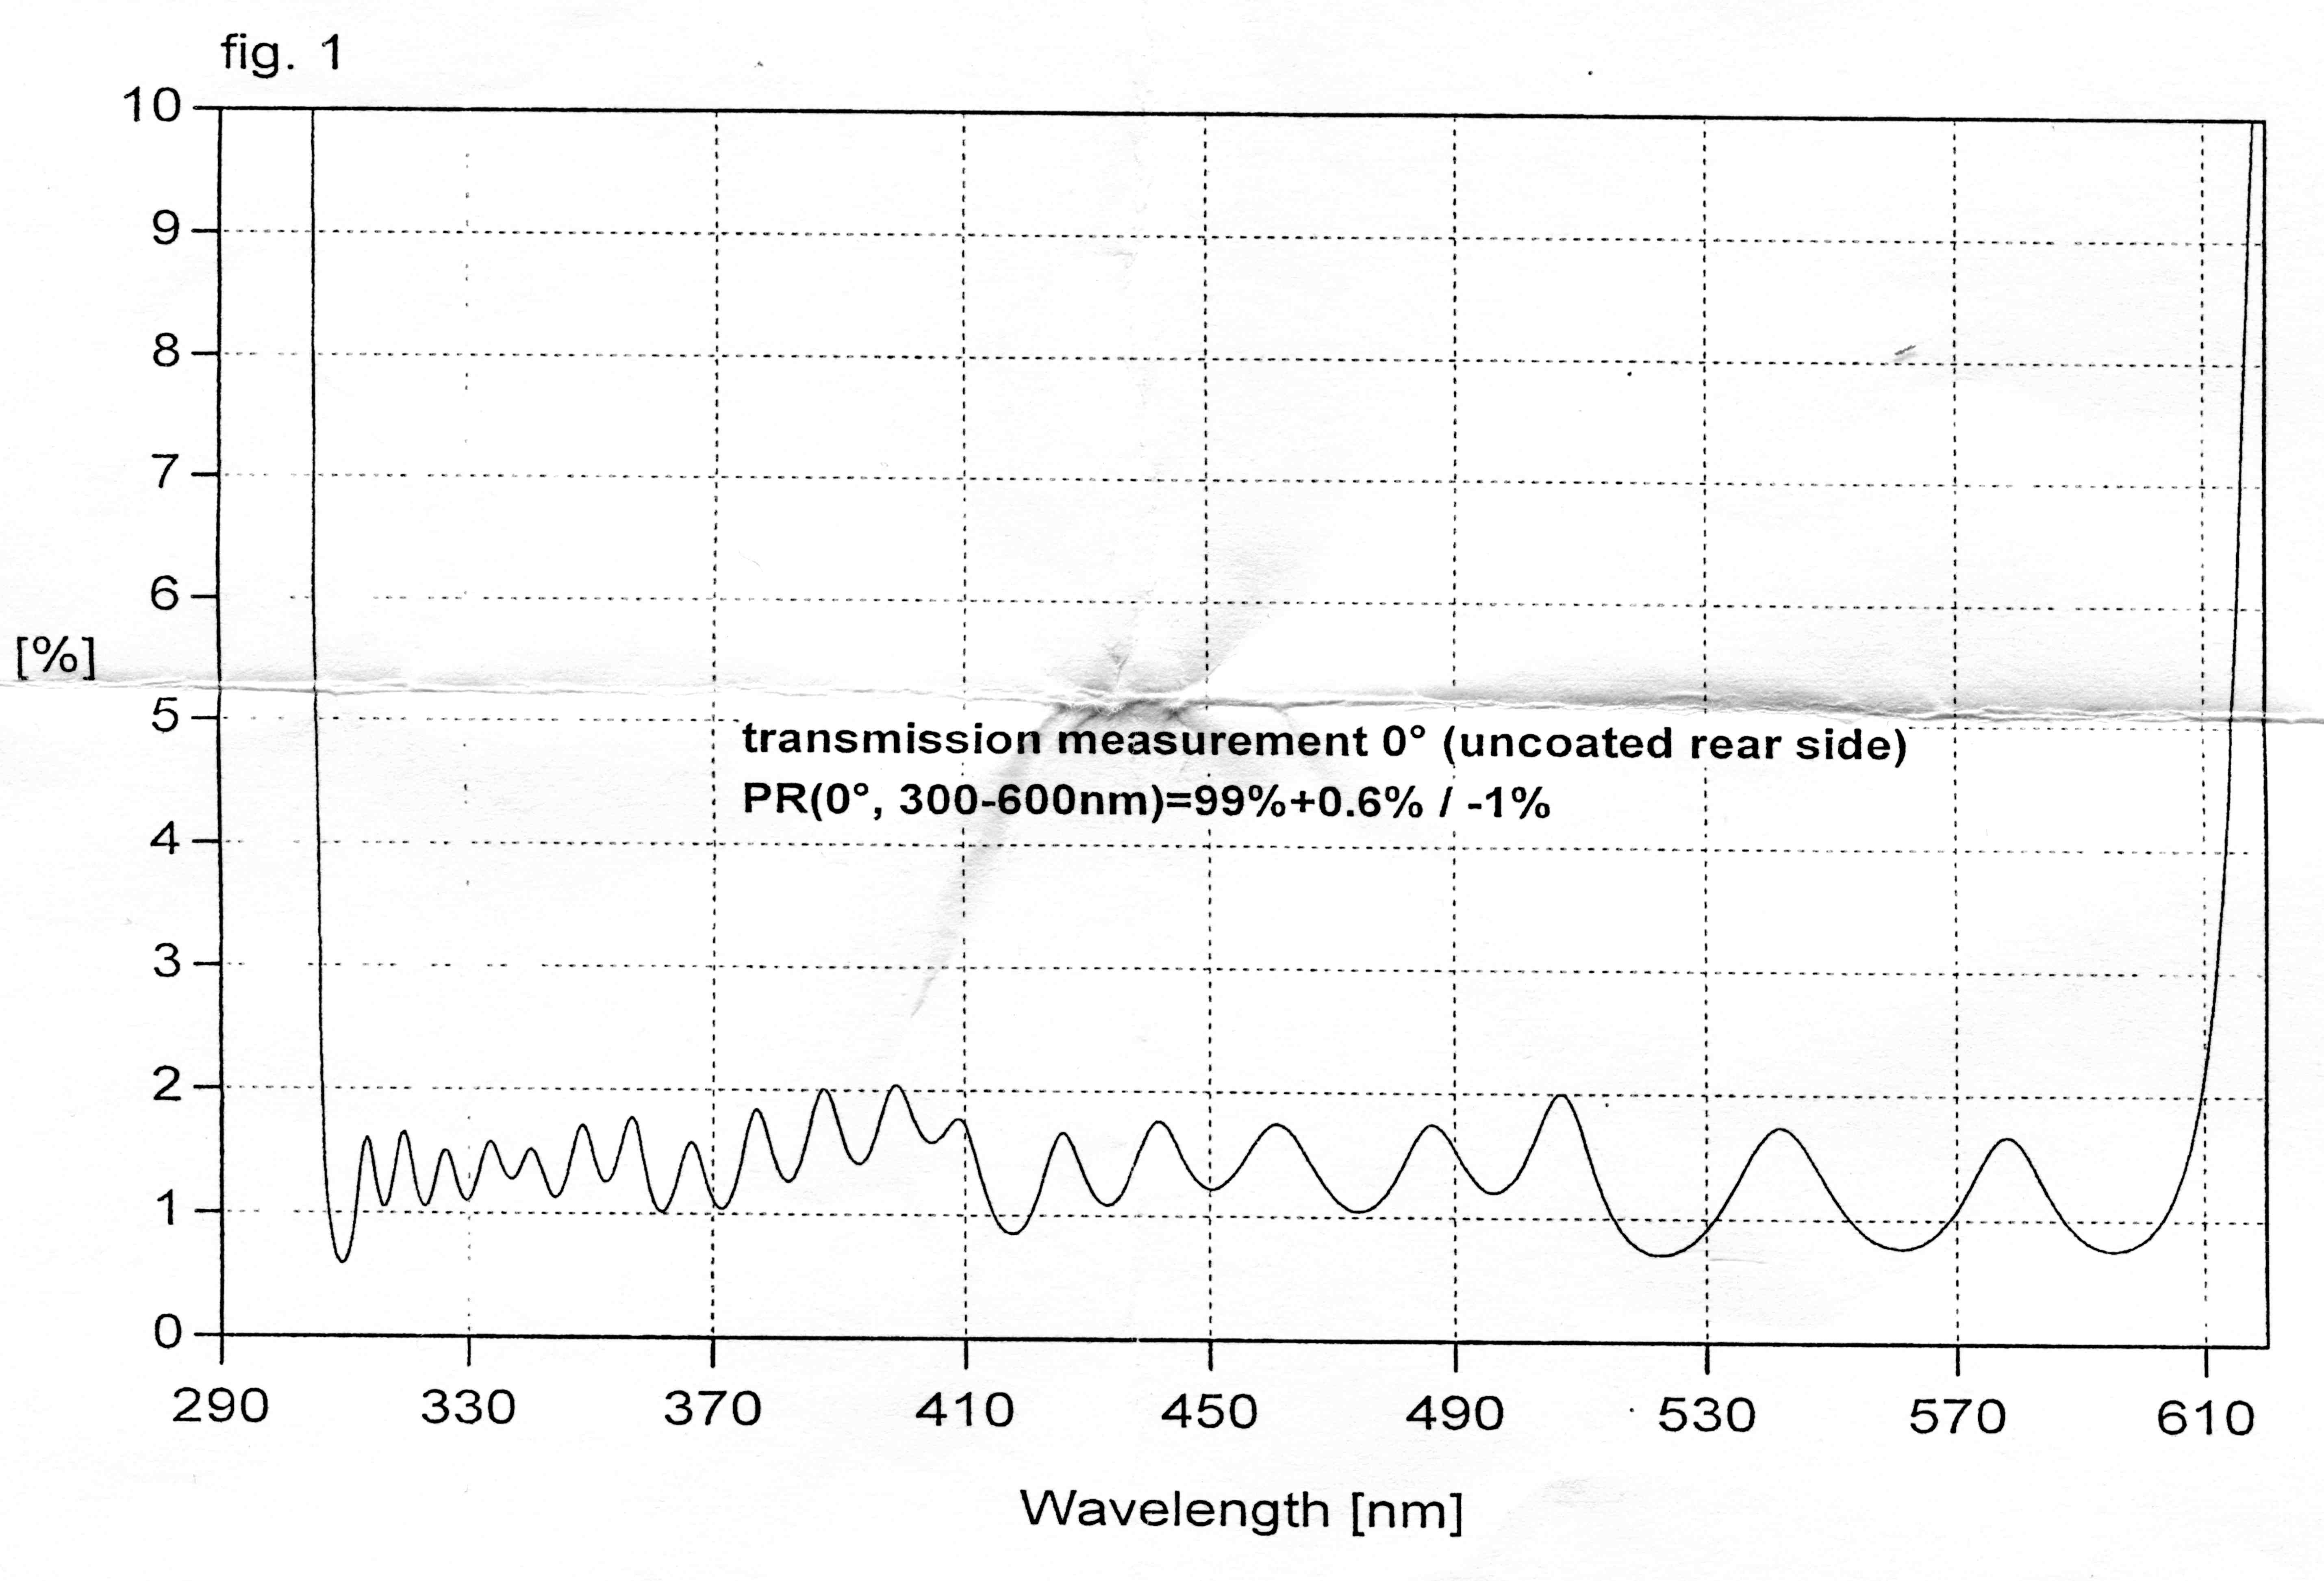
\includegraphics[width=\textwidth]{figures/mirrors.jpg}
\end{center}
\caption{The mirror reflectivity provided by the manufacturer.}
\label{fig:mirror}
\end{figure}

No matter what \ac{BBCEAS} equation an experimenter decides to use to calculate
the absorption spectrum of a sample, the mirror reflectivity must be explicitly
known, as it appears in the form of $\tfrac{1-R}{d}$ \eqref{eq:ceas_std} or in
multiple places for other equations \eqref{eq:ceas_geo_mod}. The inclusion of
$R$ in these equations represents a correction to the path length to account
for the number of passes that light undergoes once it is inside the cavity.

If one neglects to determine the mirror reflectivity of the cavity, as a
function of wavelength, then two anomalous actions occur. The simplest to
understand is that the calculated values of absorption can have an extra error
that can easily exceed error due to other sources. While a calibration against
a known concentration allows one to neglect this source of error when
attempting to determine the unknown concentration of an absorber, the values
calculated provide an inaccurate understanding of the actual absorption of a
particular electronic transition.

The second, more peculiar result of neglecting the mirror reflectivity curve is
that the calculated absorption spectrum changes in \emph{shape}, which  can
lead to both artifacts in the spectrum as well as an alteration of the shape of
a transition. Attempting to fit an accurate profile to a transition in a
spectrum would be an exercise in frustration at best.

There are two ways to determine the mirror reflectivity curves. The first is
to simply have the manufacturer provide the information, or to digitalise a
graph provided through an \ac{FTS} type measurement, although this is known to
not work very well in practice as the mirror reflectivity is a function of the
alignment of the cavity \cite{Berden:2009wk}. The second common method is to
use the \ac{BBCEAS} setup in a \ac{CRDS} experiment, which, due to the self
calibrating nature of \ac{CRDS}, allows one to extract the mirror reflectivity
curves.



\section*{Chapter Review}

While \ac{BBCEAS} does require a few calibration steps to acquire a full
understanding of the spectra it produces, these procedures are not unlike what
an experimenter would go through for a normal absorption, single pass
measurement. In addition, these considerations increase the information of
absorption spectra by characterising the noise inherent in the instrument at
each wavelength the instrument measures at, correcting for the nonlinear
effects that can occur during a measurement.

\chapter{Europium Experiments}\label{ch:eu_exp}

Previous experiments have been able to detect small quantities of liquid
europium using absorption spectroscopy in the ultraviolet \cite{Yun:2001wc}.
However, the most interesting transitions for europium occur in the visible due
to the high efficiencies of the fluorescence decay pathway in europium. Under
these conditions, it is difficult to acquire an accurate absorption spectrum
for analysis of concentration or natural radiative lifetimes. To date, it
appears that within the visible the lowest concentration ever measured is
200\,mM of aqueous europium. This has been measured using complex
spectrophotometers and through \ac{PAS} \cite{Sawada:1979vca}.

These experimental results reveal a few interesting factors about
europium's electronic transitions (see Figure~\ref{fig:eu_spec_theory}.
First, the forbidden transitions are not much weaker than the allowed
$^7F_0 \leftrightarrow ^5D_2$ transition near 464nm, which occurs when
nonlinear effects to the electronic wave functions play a dominant role
\cite{Walsh:2005te}. A second unexpected attribute was noted in the forbidden
$^7F_0 \leftrightarrow ^5D_0$ transition indicating that this absorption
peak was incredibly small in comparison to other transitions in the aqueous
europium spectrum \cite{Sawada:1979vca}. The authors who noted this
peculiarity suggests that the thinness is due to hypersensitivity of the
transition to the environment that the europium is in, leading to a squeezing
effect of the spectral line that overpowers the broadening effects.

It is important, especially for the applications discussed in
section~\ref{subsec:eu_beads}, to be able to detect aqueous europium at
much smaller concentrations than 200\,mM in the visible. As the proceeding
discussion shows, \ac{BBCEAS} is uniquely apt at being able to determine
minute quantities of aqueous europium in a way that provides qualitative
data about the fluorescence transitions that is most possible through other
methods. As such, the experimental setup designed in chapter~\ref{ch:bbceas}
was used to determine just how low of a limit of detection could be obtained
with \ac{BBCEAS}.



\section{Measurements using BBCEAS}\label{sec:eu_measurements}

\begin{figure}[t]
\begin{center}
\includegraphics[]{figures/plots/eu_conc/eu_conc.pdf}
\end{center}
\caption[Europium Absorption Spectra at different Concentrations]{Europium absorption spectrum taken at different concentrations, with w reference from Sawada 1979 \cite{Sawada:1979vca}. The peaks are noticeable even though the spectra appear different. The peculiar undulations between expected peaks are due to laser fluctuations. The shaded areas represent one standard deviation of error. The larger error near 600\,nm is due to low light intensity in that range after the 585\,nm edgepass filter.}
\label{fig:eu_conc}
\end{figure}

With experimental and theoretical results indicating what should be seen in
an absorption spectrum, the \ac{BBCEAS} technique was applied to measure
small concentrations of liquid europium in the visible, at concentrations
lower than the 200\,mM seen in the literature \cite{Sawada:1979vca}. This
was accomplished using the same technique used to perform the rhodamine 6G
calibrations in chapter \ref{ch:cal}.

As one can see from figure~\ref{fig:eu_conc}, the major electronic transitions
were easily observed. However, as one can see from the figure, it is difficult
to determine why the measured spectrum has a higher baseline, and why the
relative intensities between the transitions do not match those in the
literature. Since altering of the intensity of the a transition can occur
when a substance is optically saturated, the experiment was repeated at lower
powers.

\begin{figure}[t]
\begin{center}
  \includegraphics[]{figures/plots/eu_power/eu_power.pdf}
\end{center}
\caption[Europium Absorption Spectra at different Input Intensities]{Europium absorption spectrum taken at different powers. These spectra are cleaner than in Figure~\ref{fig:eu_conc} due to better control over the laser fluctuations. The similar shapes between input powers indicates that optical saturation was not a factor in causing the undulations in Figure~\ref{fig:eu_conc}.}
\label{fig:eu_power}
\end{figure}

Figure~\ref{fig:eu_power} debunks the idea of optical saturation because the
absorption spectra are similar at many different input powers to the cavity,
even though the highest power in the set of the experiments is the same as
the original. This peculiar result is likely due to laser fluctuations in
the original liquid europium measurements. The intensity fluctuations would
increase the intensity of the peaks relative to each other and cause some line
broadening because the the laser fluctuation is a function of time \emph{and}
wavelength: see section~\ref{subsec:laser_fluc}.

Measurements were also performed on a variety of concentrations. This resulted
in a minimal detection limit of approximately 5\,mM in the visible, a 40 fold
improvement in the limit of detection against what is commonly seen in the
literature. This sensitivity is based on equation \eqref{eq:ceas_err_geo}.

These results indicate that \ac{BBCEAS} can be used to detect liquid Eu(III)
at a lower concentration than what was possible before. With modifications to
the \ac{BBCEAS} setup discussed in section~\ref{sec:bbceas_enhance} it will be
possible to lower the detectable concentration to the micromolar range because
the major source of experimental error -- the intensity fluctuations -- will be eliminated.



\section{Further Investigations of Europium}\label{sec:eu_future}

In this chapter it has been shown that preliminary \ac{BBCEAS} testing of
Eu(III) in aqueous solution can be detected in much smaller quantities than
previously reported in the literature.  This detection limit, combined with
coordination complexes, can be used to better understand europium complexes and
to illuminate how to use such complexes effectively.



\subsection{Europium Complexes}\label{subsec:eu_complex}


\begin{wrapfigure}{o}{\marginspace}
\begin{center}
  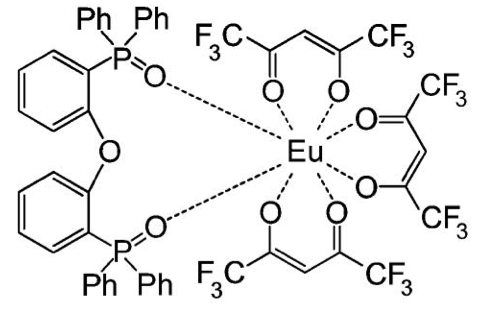
\includegraphics[width=\marginspace]{figures/eu_complex.png}
\end{center}
\emph{\footnotesize{\raggedright{A europium complex \cite{Wilson:2010hs}}}}
\end{wrapfigure}

It is quite tricky to measure the absorption spectrum of europium
and detect any fluorescence due to the extremely low absorption
cross sections of the europium ion. Coordination complexes
alleviate this problem by acting as ``catcher's mitts'', which
dramatically increase the probability of a photon being absorbed
\cite{Kirby:1983cl,Sveshnikova:2000cr,Werts:2002fs,Bunzli:2005ic,Moudam:2009in,Wilson:2010hs,Harma:2010dm,InstituteofBiomedicine:2011vt,Pihlasalo:2012cq}.
Combined with the high fluorescence quantum efficiency of the europium
complexes, these coordination systems increase the usability of europium by
allowing even moderate intensity light sources to induce fluorescence of high
spectral purity.

However, to calculate the theoretical parameters for such a system, it is
necessary to measure the time required for an excited europium complex to decay
down to the ground state. As shown from equations \eqref{eq:nat_life_emiss},
\eqref{eq:nat_life_abs} and \eqref{eq:branch_ratio}, it is possible to use the
absorption and emission spectrum of a given transition to determine the natural
radiative lifetime of the complex, transition probabilities and branching
ratios. This information is necessary to acquire a better theoretical
understanding of the electron configuration and interaction in europium
complexes. The derived theory can then be used to optimise coordination
complexes to acquire the highest fluorescence yields, or more spectrally pure
fluorescence by the reduction or enhancement of certain electron dipole
transitions. This information could be useful to engineers attempting to design
\acp{OLED}, as they could engineer the intensity and spectral bands at which
the complexes would fluoresce.



\subsection{Europium Complexes adsorbed to Polystyrene Beads}\label{subsec:eu_beads}

\begin{figure}[t]
\begin{center}
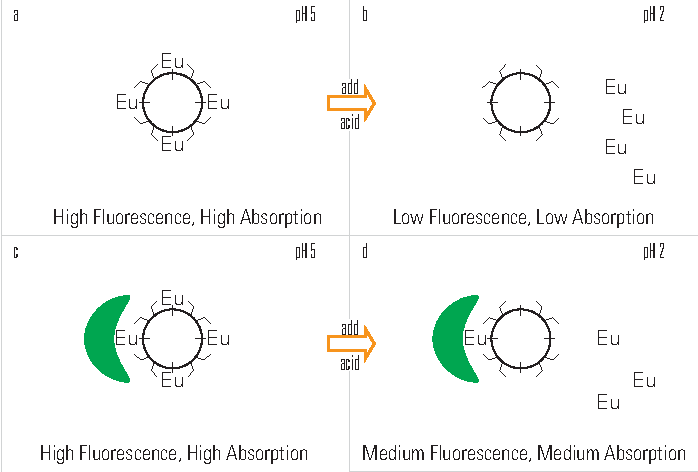
\includegraphics[]{figures/eu_beads/eu_beads.pdf}
\end{center}
\caption[Europium Bead Protein Assay]{When polystyrene beads coated with europium complexes (a) are exposed to an acidic environment (b), the complexes dissolve, reducing the absorption and fluorescence signal given off by europium. If, however, a biomolecule is adhered to the surface (through ionic interactions, c), then the europium under the molecule is prevented from leaving its complex (d). This keeps the absorption and fluorescence signals high, and how high these signals are can be used to determine both the quantity of biomolecules in a solution on a molecule by molecule basis.}
\label{fig:eu_beads}
\end{figure}

Europium complexes have been used as fluorescent markers and for displays,
among other applications. However, a recent paper provides an interesting use
of europium complexes attached to nano polystyrene beads. These beads are able
to hold tens of thousands of chelated europium complexes on one bead. While
this is interesting on its own as a way to produce highly localised intense
fluorescence, the beads also have an additional property that makes them useful
for detections of larger biomolecules and cells: the beads are designed with a
negative surface potential, even with the europium complexes attached.

This is useful because many proteins and cells will adhere to the surface of
the beads. If a europium ion attempts to disassociate from its coordination
complex, it is sterically hindered from doing so. In highly acidic solutions --
around a pH of 2 -- europium tends to disassociate from its complex readily,
which reduces the fluorescence signal. However, since attached biomolecules
prevent this dissociation through steric hindrance, it is possible to use the
ratio of the observed fluorescence in a biomolecule solution to the background
fluorescence upon all the complexes dissociating to calculate the amount of a
biomolecule there is in a solution.

Detecting the concentration of a biomolecule is currently done using
fluorescence properties of europium complexes. However, absorption techniques
can lead to higher sensitivities and lower limits of detection because the
absorption measurement does not need to account for a large scattering
angle, unlike fluorescence where an emitted photon could travel in any
direction.\marginpar{This is to say it is easier to detect the reduction of
photons due to absorption than it is to pray that an emitted photon will
travel in the correct direction.} As such, a \ac{BBCEAS} measurement of the
absorption spectrum of a biomolecule solution laced with europium complexes
should lead to even greater sensitivities and lower limits of detection than
currently stated in the literature.

Additionally, the speed of \ac{BBCEAS} measurements would greatly decrease the
time required to acquire biomolecule concentrations to only a few minutes.
Besides the clear advantage of fast molecular concentration determination, the
fast acquisition of the absorption spectrum allows for detection limits that
are lower than the fluorescence measurements by measuring the \emph{rate
constant} for the decay process. In this manner, even concentrations of
biomolecules that did not create a significant shift from no biomolecule
samples could still be determined using the slow down of the decay of the
absorption signal versus a blank sample.

Extra benefits can be found from the property that the electronic dipole
transitions in europium complexes will alter due to the adsorption of a
biomolecule onto the bead. Judd-Ofelt theory allows for many of the forbidden
transitions provided a higher order interaction with a localised electric
field, which can come from a complex or the surrounding medium. As such,
parameters such as the branching ratio and natural radiative lifetime would be
affected by the biomolecule attached to the europium bead. This would prove to
be a novel approach to not only detecting minuscule concentrations of proteins
in a solution, but would also allow for the adsorbed protein on the beads to
be identified. It is feasible to believe that this identification process
could be done to multiple biomolecules simultaneously, creating a single
molecular probe for determining the concentrations of different proteins in a
molecular soup, such as a cell lysate sample.

With the ability to achieve lower limits of detection, higher sensitivities,
fast acquisition and biomolecule identification, \ac{BBCEAS} detection of
europium complex beads provides a tantalising alternative to traditional
biomolecule detection techniques. \ac{BBCEAS} could be integrated into
microtiter pipette plates to provide an all in one solution for rapidly
testing concentrations of cell lysates or other samples.



\section*{Chapter Review}

Europium is a complicated metal. It is difficult to detect in a solution,
readily reacts with its neighbors, and is only partially understood from a
theoretical basis. However, the \ac{BBCEAS} technique created in chapter
\ref{ch:bbceas} has proven to be useful in both in lowering the limit of
detection for aqueous europium and in acquiring useful, broad spectra that
can be used to calculate parameters such as the natural radiative lifetime of
a transition. With the work laid out in this chapter, it will be possible to
combine \ac{BBCEAS} with europium complexes to create truly amazing protein
assays that detect not only minuscule quantities of proteins but can also
identify which proteins are in a solution.

\chapter{Conclusion} \label{ch:discussion}

The work documented in this report was performed for two reasons. One was to
investigate \ac{BBCEAS} as an experimental technique, and to explore possible
modifications that would increase the sensitivity and repeatability of spectra
measured from a \ac{BBCEAS} setup. This technique was then used for the second
piece of work investigating the electronic transitions of aqueous europium and
what kind of ways \ac{BBCEAS} and europium could be combined.

The results obtained from investigating \ac{BBCEAS} are promising.
A reliable way of calculating and visualising error was crafted in
section~\ref{subsec:ceas_error}, and from creating the layout in
section~\ref{sec:optical_layout}, potential improvements were identified. In
addition, the effects of several sources of error were investigated in chapter
~\ref{ch:cal}. Through this investigation, a new file format named
\emph{CamTIFF} and a spectroscopic software suite called \emph{Apollo} were
created to simplify experimental design and work.

Building on this \ac{BBCEAS} framework, absorption spectra of europium
ions were detected to validate previous results in the literature,
as well as to investigate the potential uses of aqueous europium. A
theoretical understanding of europium's electronic configuration and the
implications of this to the observed absorption spectra were investigated in
chapter~\ref{ch:eu_theory}, and preliminary absorption spectra were obtained
in chapter~\ref{ch:eu_exp}.



\section*{Future Work}

\acl{BBCEAS} is a simple spectroscopic technique that in most cases is
used as a way to measure the concentration of an analyte in a solution.
This description tends to minimise a technique that can offer a greater
understanding of difficult theoretical and experimental questions. \ac{BBCEAS}
can probe electronic transitions that are otherwise impossible to detect with
other absorption techniques, and its spectrally wide results can be used to
understand the longevity of an excited state. This information can be used to
create efficient assays that provide solution specific spectroscopic values
that can be used not only to determine the concentration of an analyte but
to identify molecules in a solution that would otherwise be difficult or
impossible with other spectroscopic methods. In addition, the simplicity of
\ac{BBCEAS} allows it to be easily commercialised into a small, cheap and yet
potent form factor.

\begin{wrapfigure}{o}{\marginspace}
\begin{center}
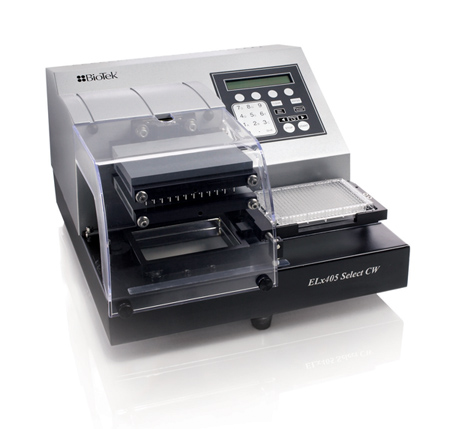
\includegraphics[width=\marginspace]{figures/microtiter_machine.jpeg}
\end{center}
\emph{\footnotesize{ A potential automatic protein assay machine that works on microtiter well plates. This would allow for many permutations of an analyte to be tested quickly and efficiently. Courtesy Wikipedia.}}
\label{fig:microtiter}
\end{wrapfigure}

The inherent utility of \ac{BBCEAS} can be combined with the fluorescence
properties of europium based coordination complexes to yield truly astonishing
assays. Adding small concentrations of europium laden polystyrene beads to
an unknown molecular soup would allow an experimenter, using \ac{BBCEAS}, to
pick out vanishingly small quantities of proteins and other large biomolecules
from a solution due to the fact that the spectra acquired would alter in both
general shape and amplitudes in response to different analytes. This would
allow experimenters to build a table of known spectra of aqueous europium
complexes in the presence of certain molecules that could be used to fingerprint molecules in aqueous solutions.

The process of creating molecule specific assays could be performed
automatically and in a microtiter plate. This would allow biologists and
chemists to run many experimental permutations simultaneously and allow
them to quickly read out the contents of the solutions that result from
the experiments performed. This analytical power would be cost effective
to manufacture, as most of the parts already exist and at low costs if
inexpensive light sources and detectors are used.

In addition to protein assays, \ac{BBCEAS} can be used to create efficient
\acp{OLED} out of europium complexes that are tailored to meet certain
spectral purity and output. The knowledge of how an excited electronic
transition can decay and how to optimise this decay can be determined
using the absorption spectra from \ac{BBCEAS} combined with a fluorescence
spectrometer.

It is easy to see that combining \ac{BBCEAS} with europium complexes can lead
to novel and effective applications in many fields, especially biomedical
research. These ideas are not unrealistic; from the work shown in this report
it is clear that these ideas could be realised in the near future without
requiring any more research apparatus than what can already be easily built.
The knowledge contained in this report paves the path for a generation of
highly sensitive, fast spectroscopic techniques that can be implemented easily
and cost effectively to assist scientists and medical personnel in their
research and diagnoses in a way not currently possible.

\cleardoublepage
%\include{Chapters/Chapter02}
% ********************************************************************
% Backmatter
%*******************************************************
\appendix
\cleardoublepage
\part{Appendix}
\chapter{CEAS Error Derivation}

    For a random variable $X$, the standard error is defined by the square root of the second moment (also known as the standard deviation) divided by the number of elements taken of $X$, represented by $x$.

    \begin{align*}
      \Delta_x = \frac{\sigma_x}{\sqrt{n}}
    \end{align*}

    We estimate the standard error in a function $f$ of $X$ by taking the partial differential of function with respect to $X$. This is known as the \emph{delta method}.

    \begin{align*}
      \Delta_f^2 =  \left( \frac{\partial f(x)}{\partial x} \Delta_x\right)^2
    \end{align*}

    This is a measure of the standard error of the mean value, which is calculated by plugging the mean value $\overline{x}$ into $f$.

    For a function $g$ of multiple independent variables $X_1,X_2,...,X_n$ we can estimate the standard error $\Delta_g$ in the following way.
    \marginpar{\\\bigskip if the variables are not independent we should add a covariance term.}

    \begin{align*}
      \Delta_g^2 = \sum_i^n\left(\frac{\partial f}{\partial x_i}\Delta x_i\right)^2
    \end{align*}

    In calculating the absorption in a CEAS experiment it is common to use the function

    \begin{align}
      \alpha(\lambda) = \left(\frac{I_0(\lambda)}{I(\lambda)}-1\right)\left(\frac{1-R(\lambda)}{d}\right)\label{eq:ceas}
    \end{align}

    where $I$ and $I_0$ represent the intensity of the light through the cavity with and without the absorber present, respectively.

    To calculate the squared error $\Delta_\alpha^2$, we shall use the delta method as defined above.
    \marginpar{$\lambda$ is omitted in the CEAS equation from now on for convenience}

    \begin{align*}
      \Delta_\alpha^2 &= \left(\frac{\partial \alpha}{\partial I_0}\Delta_{I_0}\right)^2  + \left(\frac{\partial \alpha}{\partial I}\Delta_I\right)^2  \\\\
                      &= \left[\frac{\Delta_{I_0}}{I}\left(\frac{1-R}{d}\right)\right]^2 + \left[\frac{I_0 \Delta_I }{I^2}\left(\frac{1-R}{d}\right)\right]^2 \\\\
                      &= \left(\frac{\Delta_{I_0}}{I} + \frac{I_0\Delta_I}{I^2}\right)^2 \left(\frac{1-R}{d}\right)^2 \\\\
               &= \left[\left(\frac{\Delta_{I_0}}{I} + \frac{I_0\Delta_I}{I^2}\right) \left(\frac{1-R}{d}\right)\right]^2
    \end{align*}

    This can be simplified to get the standard error.
    \begin{align}
      \Delta_\alpha = \left(\frac{\Delta_{I_0}}{I} + \frac{I_0\Delta_I}{I^2}\right) \left(\frac{1-R}{d}\right)\label{eq:err}
    \end{align}

    This CEAS equation assumes that the reflectivity is close to 1 and that $\alpha$ is nearly zero (only weak, low concentration absorbers). A version of this equation that does not make this assumption is shown below.

    \begin{align}
      \alpha = \frac{1}{d}\left|\ln\left(\frac{1}{2R^2}\left(\sqrt{4R^2+\left(\frac{I_0}{I}(R^2-1)\right)^2} + \frac{I_0}{I}(R^2-1)\right)\right)\right| \label{eq:ceas_full}
    \end{align}

    Here we will introduce, for convenience, two simplifications
    \begin{align*}
      \zeta &= \ln\left(\frac{1}{2R^2}\left(\sqrt{4R^2+\left(\frac{I_0}{I}(R^2-1)\right)^2} + \frac{I_0}{I}(R^2-1)\right)\right)\\\\
      \beta &= \sqrt{4R^2+\left(\frac{I_0}{I}(R^2-1)\right)^2}
    \end{align*}

    Hence
    \begin{align*}
      \alpha = \frac{1}{d}\left|\ln\left(\frac{1}{2R^2}\left(\beta+\frac{I_0}{I}(R^2-1)\right)\right)\right| = \frac{\left|\zeta\right|}{d}
    \end{align*}

    Now, we can easily find the partials
    \begin{align*}
      \frac{\partial \alpha}{\partial I_0} &= \text{sgn}(\zeta)\left(\dfrac{1}{I}\right)\left(\dfrac{R^2-1}{d\beta}\right)\\\\
        \frac{\partial \alpha}{\partial I} &= -\text{sgn}(\zeta)\left(\dfrac{I_0}{I^2}\right)\left(\dfrac{R^2-1}{d\beta}\right)
    \end{align*}

    After which we can easily estimate the standard error in $\alpha$.

    \begin{align*}
      \Delta_\alpha^2 &= \left(\frac{\partial \alpha}{\partial I_0} \Delta_{I_0}\right)^2  + \left(\frac{\partial \alpha}{\partial I} \Delta_{I}\right)^2 \\\\
                      &= \left(\frac{\Delta_{I_0}}{I} + \frac{I_0\Delta_{I}}{I^2}\right)^2 \left(\dfrac{R^2-1}{d\beta}\right)^2 \\\\
                      &= \left[\left(\frac{\Delta_{I_0}}{I} + \frac{I_0\Delta_{I}}{I^2}\right)\left(\dfrac{R^2-1}{d\beta}\right)\right]^2 \text{ given $\alpha \neq 0$}
    \end{align*}

    The sign function has been removed because it was squared, which results in a multiplication by one unless $\alpha$ is zero, at which point the error is also zero.\marginpar{\\\vspace{-3em}However, be careful when $I$ is zero!}

    Finally, this can be simplified to the standard error
    \marginpar{\\\bigskip One can use the standard deviation instead of standard error without loss of generality.}

    \begin{align}
      \Delta_\alpha &= \left(\frac{\Delta_{I_0}}{I} + \frac{I_0\Delta_{I}}{I^2}\right) \left(\dfrac{R^2-1}{d\beta}\right) \notag\\\notag\\
                    &= \left(\frac{\Delta_{I_0}}{I} + \frac{I_0\Delta_{I}}{I^2}\right) \left(\dfrac{R^2-1}{d}\right)\left(4R^2+\left(\frac{I_0}{I}(R^2-1)\right)^2\right)^{-1/2} \label{eq:err_full}
    \end{align}
    {\color{Maroon}{Equations \eqref{eq:ceas_full} and \eqref{eq:err_full} are preferred to \eqref{eq:ceas} and \eqref{eq:err} because neither \eqref{eq:ceas_full} nor \eqref{eq:err_full} make assumptions on the limits of $R$ or $\alpha$, whereas \eqref{eq:ceas} and \eqref{eq:err} do make the assumptions $R \to 1$ and $\alpha \to 0$.}}


%\chapter{CamTIFF}


\chapter{Software Listings}

%********************************************************************
% Other Stuff in the Back
%*******************************************************
\cleardoublepage%********************************************************************
% Bibliography
%*******************************************************
% work-around to have small caps also here in the headline
\manualmark
\markboth{\spacedlowsmallcaps{\bibname}}{\spacedlowsmallcaps{\bibname}} % work-around to have small caps also
%\phantomsection
\refstepcounter{dummy}
\addtocontents{toc}{\protect\vspace{\beforebibskip}} % to have the bib a bit from the rest in the toc
\addcontentsline{toc}{chapter}{\tocEntry{\bibname}}
\bibliographystyle{unsrt}
\label{app:bibliography}
\bibliography{bibliography}

\cleardoublepage\pagestyle{empty}

%\begin{flushright}{\slshape
    %We have seen that computer programming is an art, \\
    %because it applies accumulated knowledge to the world, \\
    %because it requires skill and ingenuity, and especially \\
    %because it produces objects of beauty.} \\ \medskip
    %--- Donald E. Knuth
%\end{flushright}

\hfill

\vfill

\begingroup
%\pdfbookmark[0]{Colophon}{colophon}
%\section*{Colophon}
\noindent This document was typeset using the typographical look-and-feel \texttt{classicthesis} developed by Andr\'e Miede.
The style was inspired by Robert Bringhurst's seminal book on typography ``\emph{The Elements of Typographic Style}''.
\texttt{classicthesis} is available for both \LaTeX\ and \mLyX:
\begin{center}
\url{http://code.google.com/p/classicthesis/}
\end{center}

\bigskip

\noindent\finalVersionString
\endgroup


\cleardoublepage%*******************************************************
% Declaration
%*******************************************************
\refstepcounter{dummy}
\pdfbookmark[0]{Declaration}{declaration}
\chapter*{Declaration}
\thispagestyle{empty}
We hereby approve the dissertation of \emph{\myName}, candidate for the degree of \emph{Masters of Philosophy by Research}.
\bigskip

\noindent\textit{\myLocation, \myTime}

\smallskip

\begin{flushright}
    \begin{tabular}{m{5cm}}
        \\ \hline
        \centering\spacedlowsmallcaps{Professor \myProf} \\
    \end{tabular}

    \bigskip

    \begin{tabular}{m{5cm}}
        \\ \hline
        \centering\spacedlowsmallcaps{Examiner 1} \\
    \end{tabular}

    \begin{tabular}{m{5cm}}
        \\ \hline
        \centering\spacedlowsmallcaps{Examiner 2} \\
    \end{tabular}

\end{flushright}

% ********************************************************************
% Game Over: Restore, Restart, or Quit?
%*******************************************************
\end{document}
% ********************************************************************
